% ---------------------------------------------------------------------------
% Dual-Bottleneck Agents
%
% Batch 2: real figures and tables wired in.
%   - \includegraphics for all 12 published figures (figures_zh/ is self-contained
%     so the paper/ directory can be uploaded to Overleaf as-is)
%   - booktabs tables built from reports/paper_data_final/tables/*.md
%   - figure captions below, table captions above (NeurIPS convention)
%   - \label on every float; cite them with \ref, never with a hard-coded number
%
% Abstract / Introduction / Section 3 are verbatim author text.
% Sections 4-8 carry no body prose yet: the prose was not supplied.
%
% Compile target: pdfLaTeX (works unchanged on Overleaf).
% ---------------------------------------------------------------------------

% ---------------------------------------------------------------------------
% NeurIPS 2026 官方模板。
% 注意：neurips_2026.sty 内部已经 RequirePackage 了 geometry / natbib / hyperref，
% 因此下面这几行不能再各自加载，否则会 option clash 直接报错。
% 原先的 \documentclass[11pt]{article} 与 \usepackage[margin=1in]{geometry}
% 会让版面变成单栏 1 英寸边距，与 NeurIPS 双栏模板冲突，已移除。
% ---------------------------------------------------------------------------
\documentclass{article}
% natbib is loaded by neurips_2026.sty via \RequirePackage{natbib} with no
% options, which defaults to author-year. Passing the options here is the
% mechanism the style file itself documents, so numeral citations work
% without touching the style file.
\PassOptionsToPackage{numbers,compress}{natbib}
\usepackage[preprint]{neurips_2026}

% ---------------------------------------------------------------------------
% 中文排版支持（本次翻译新增；英文原版 main.tex 无此块）
% 中文必须用 XeLaTeX 或 LuaLaTeX 编译，pdflatex 无法直接排中文：
%   xelatex main_zh.tex
% 若 ctex 与 neurips_2026.sty 的字体设置冲突，改用下方注释掉的 xeCJK 方案。
% ---------------------------------------------------------------------------
\usepackage[UTF8]{ctex}
% \usepackage{xeCJK}
% \setCJKmainfont{Noto Serif CJK SC}
% \setCJKsansfont{Noto Sans CJK SC}

% ---------------------------------------------------------------------------
% 中文版规范之一：摘要标题必须是「摘要」，正文写 \begin{摘要}...\end{摘要}。
% 标准 LaTeX/ctex 没有名为「摘要」的环境，因此这里自行定义。
% 之所以不复用 neurips_2026.sty 的 abstract 环境：该样式的标题文字可能是硬编码的
% 英文 "Abstract"，用别名 + \abstractname 未必覆盖得到（本机没有该 .sty，无法验证）。
% 自建环境能保证标题一定显示为「摘要」。
% 若希望沿用样式的摘要版式、只改标题文字，把下面这段换成注释里的别名方案。
% ---------------------------------------------------------------------------
\makeatletter
\@ifundefined{摘要}{%
  \newenvironment{摘要}{%
    \par\addvspace{0.8\baselineskip}%
    \begin{center}\large\bfseries 摘要\end{center}%
    \addvspace{0.3\baselineskip}%
    \begingroup\leftskip=1.5em\rightskip=1.5em\noindent\ignorespaces
  }{%
    \par\endgroup\addvspace{0.8\baselineskip}%
  }%
}{}
\makeatother
% 别名方案（备选）：
% \makeatletter
% \@ifundefined{摘要}{\newenvironment{摘要}{\begin{abstract}}{\end{abstract}}}{}
% \makeatother
% \providecommand{\abstractname}{摘要}\renewcommand{\abstractname}{摘要}
% ---------------------------------------------------------------------------

% ---------------------------------------------------------------------------
% 页数控制：中文版正文必须与英文版同为 9 页（NeurIPS 正文上限 9 页）。
%
% 实测（不是估算）——从两份已编译 PDF 的文本基线间距量得：
%   未压缩（中文版.pdf, 14:47）     汉字行距 16.4 pt
%   已压缩（20:12 那份）           汉字行距 14.8 pt
% ctex 的汉字行距 = 1.30 x \@setfontsize 的第二参数（14.8 / 11.4 = 1.298），
% 所以第一参数只改字号，第二参数才是真正控制行距的旋钮。
%
% 版面账（20:12 那份 PDF，文本区高 679.5 pt/页）：
%   正文 = 10 页整，参考文献标题落在第 11 页 y=72.6pt，即页顶 9.2% 处。
%   10 页里图片占 543.8 pt（8.0%），其余 6251.2 pt 是可压缩的散文/公式。
%   要落进 9 页，散文必须压到 5571.7 pt，系数 0.8913。
%   竖向高度约等于 字号 x 行距，等比缩放 f 时高度按 f^2 收缩，
%   故 f = sqrt(0.8913) = 0.944；这里取 0.94 留一点余量（预计 8.9 页，
%   浮动体可能迁移位置，留余量免得正好卡在 9 页边界上）。
%
% 唯一需要调的旋钮：\ZHFontSize / \ZHLeading，两者同乘一个 f。
%   当前 f = 0.94：字号 9.98 -> 9.38 pt，第二参数 11.4 -> 10.72 pt
%   （汉字行距随之 14.8 -> 13.94 pt，汉字行距/字号仍为 1.485，不会上下相碰）
% 编译后若仍不是 9 页：
%   偏多 -> f 再乘 0.98（两个数一起乘）；偏小/想放大 -> f 乘 1.02。
% 想彻底关掉压缩、回到 ctex 默认：注释掉 \def\ZHPageCompact{1} 那行。
%
% 校验工具：python paper/_zh_pagecount.py --pdf <编译产物>.pdf
%   它会直接量出正文占几页、图片占多少、以及还需要多大的 f，不用靠猜。
% ---------------------------------------------------------------------------
\makeatletter
\def\ZHPageCompact{1}%
\ifx\ZHPageCompact\@undefined\else
\AtBeginDocument{%
  \renewcommand\normalsize{%
    \@setfontsize\normalsize{9.38}{10.72}%
    \abovedisplayskip 8\p@ \@plus2\p@ \@minus4\p@
    \abovedisplayshortskip \z@ \@plus2\p@
    \belowdisplayshortskip 4\p@ \@plus2\p@ \@minus2\p@
    \belowdisplayskip \abovedisplayskip
    \let\@listi\@listI}%
  \normalsize
}%
\fi
\makeatother
% ---------------------------------------------------------------------------


% --- encoding and fonts -----------------------------------------------------
\usepackage[utf8]{inputenc}
\usepackage[T1]{fontenc}

% --- math -------------------------------------------------------------------
\usepackage{amsmath}
\usepackage{amssymb}

% --- figures and tables -----------------------------------------------------
\usepackage{graphicx}
\usepackage{booktabs}
\usepackage{tabularx}
\usepackage{array}

% --- bibliography -----------------------------------------------------------
% natbib 由 neurips_2026.sty 内部加载，此处不再重复；数字模式用
% \PassOptionsToPackage{numbers,compress}{natbib} 传入（见文件开头）。
% neurips_2026.sty 本身不设 \bibliographystyle，必须由正文提供；
% 文末用 unsrtnat 让文献编号按首次引用顺序排列（plainnat 按作者字母序）。

% ---------------------------------------------------------------------------
\title{《双重瓶颈：自进化智能体中裁判可靠度与生成器能力的合成律》}
\author{李 浩\\[2pt]\small 独立研究者\\[2pt]\small \texttt{lihao9108@outlook.com}}
\date{\today}
% ---------------------------------------------------------------------------

% Equation spacing (global preamble settings; no per-equation \vspace).
\setlength{\abovedisplayskip}{6pt plus 2pt minus 2pt}
\setlength{\belowdisplayskip}{6pt plus 2pt minus 2pt}
\setlength{\abovedisplayshortskip}{3pt plus 1pt minus 1pt}
\setlength{\belowdisplayshortskip}{3pt plus 1pt minus 1pt}

% Float pages: \@fptop defaults to "0pt plus 1fil", which stretches a float down
% from the top of a float page. Pinning it to 0pt sets floats flush with the top
% of the text block. Preamble-only; no float-separation length is touched.
\makeatletter
\setlength{\@fptop}{0pt}
\makeatother

% Float quota per page. The LaTeX default is two top floats per page, which is
% what defers Appendix D's third table (D.5) to the page after D.3/D.4. Raising
% the quota lets D.3, D.4 and D.5 share one page. Both the single-column and the
% double-column counters are raised, since figure*/table* pick between them
% according to the column mode. Counters only; no length or fraction is touched.
\setcounter{topnumber}{3}
\setcounter{dbltopnumber}{3}
\setcounter{totalnumber}{4}

\begin{document}

\maketitle

% ===========================================================================
% ABSTRACT
% ===========================================================================
\begin{摘要}
自进化智能体（self-evolving agent）——即迭代地生成任务、求解任务并蒸馏经验的系统——在代码生成与数学推理任务上已展现出潜力。已有工作主要聚焦于裁判（judge），也就是提供反馈的评估者，并默认裁判只要足够可靠便万事大吉。通过在 Z3 约束求解任务上开展的 2,400 组受控实验，发现了第二个同等关键的瓶颈：生成器（generator），即撰写新任务的 LLM。把双重瓶颈（dual bottleneck）形式化为一条作用于误差预算（error budget）的合成律（composition law），其中生成侧（$\Delta_t^{\mathrm{gen}}$）、裁判侧（$\Delta_t^{\mathrm{valid}}$）与端到端（$\Delta_t^{\mathrm{global}}$）三个失败率相乘合成：$1 - \Delta_t^{\mathrm{global}} = (1 - \Delta_t^{\mathrm{gen}})(1 - \Delta_t^{\mathrm{valid}})$，并在 2,400 轮真实 API 实验上验证到机器精度（1.11e-16）。这条定律意味着生成器与裁判这两个瓶颈共享同一份预算：对于 $\Delta_t^{\mathrm{gen}}$ 较大的条件（condition），若要求总体容差不变，就需要更可靠的裁判；而如果 $\Delta_t^{\mathrm{gen}}$ 本身已经超出预算，那么任何裁判可靠度（judge reliability）都无法补偿。使用真实的 DeepSeek V4 Flash API 在 Level 1 任务上实测得到临界裁判可靠度 $\tau_c \approx 0.55$，并推导出无参数设计规则 $\tau_c = \sqrt{1-2\Delta_t^{\max}}$：它给出把端到端偏差控制在容忍上界 $\Delta_t^{\max}$ 之内所需的最低裁判可靠度。识别出伪难度陷阱（pseudo-difficulty trap）：当难度控制器（difficulty controller）升级到 Level 2/3 时，LLM 的任务生成有效率（valid task rate）从 $\sim$89\% 暴跌到 $<$10\%，致使系统空转、毫无进展。提出一个四层约束生成框架（four-layer constraint generation framework），并说明其中承重的是前两层——JSON 骨架与确定性渲染器——它们在真实 API 上把有效率恢复到 L1 的 100\%、L2 的 73.8\% 与 L3 的 83.8\%。
\end{摘要}

% ===========================================================================
% 1. INTRODUCTION
% ===========================================================================
\section{引言}

自进化智能体——即迭代地生成任务、求解任务并蒸馏经验的系统——已成为持续改进的一条有前景的范式。主流叙事聚焦于\textit{裁判}：如何提供可靠反馈，以防止智能体漂移进自我确认的循环。

这种担忧是有根据的。\textbf{自验证悬崖（self-verification cliff）}~\cite{self_verification_cliff}表明，生成器越强，其自选择（self-selection）缺口就越大：GPT-5.4-mini 能解出 54.7\% 的 AIME 问题，但自选择正确的比例只有 41.9\%，仅回收了其采样余量（sampling headroom）的 36\%。\textbf{Ratchet}~\cite{ratchet}给出了一个精确界：若裁判把失败判为通过的比例达到 $(1-\tau)/2$ 或更高，那么无论样本量多大，技能退役（skill retirement）都不会淘汰任何东西。\textbf{AgentJudgeBench}~\cite{agentjudgebench}揭示，LLM 裁判在困难查询上会收敛到 77--82\% 的准确率天花板，且与模型规模无关。

最初也持同样的前提。构建了一个自进化智能体，配备形式化锚定（formal anchoring，Z3）、基于种群的难度自适应以及经验蒸馏（distillation）。跑了 2,400 轮受控实验（4 个条件 $\times$ 200 轮 $\times$ 3 次重复运行）。

\textbf{原本预期能证实形式化锚定可以抑制自评分漂移，事实也确实如此}：条件 A（LLM 自评分）在 200 轮中把评估偏差（evaluation bias）$\Delta_t = 0.15$ 保持住，而条件 B（Z3 锚定）保持在 $0.00$。\textbf{但也发现了意料之外的现象}：条件 C（仅种群博弈）与条件 D（完整系统）分别使 85.5\% 与 90.5\% 的任务失效。控制器把 Level-1 的高成功率读作"已就绪"，于是升级到 Level 2/3；而在那里 LLM 无法生成有效的 Z3 代码——于是系统空转、毫无进展，把 API 预算烧在了从未走到验证环节的任务上。

\textbf{这就是伪难度陷阱。}它不是裁判失效——Z3 完全可靠。它是\textit{生成器}失效。而它揭示出：自进化系统面对的是\textbf{两个相互独立的瓶颈}，而不是一个：

\begin{enumerate}
  \item \textbf{裁判侧瓶颈}：当裁判可靠度 $\tau$ 跌破临界阈值（critical threshold）$\tau_c$ 时，累积的经验中就会含有被污染的信号。
  \item \textbf{生成器侧瓶颈}：当生成器有效率 $V$——即产出任务通过形式化验证器的轮次占比——跌破临界值 $V_c$ 时，任何难度升级都会把系统推入空转。
\end{enumerate}

单看任何一个瓶颈都无法解释这次失败。裁判再完美，也救不了一个生成器无法产出有效任务的系统。生成器再完美，也救不了一个裁判只给出噪声信号的系统。\textbf{两个瓶颈会复合。}

为了量化这一点，通过向 Z3 裁决（verdict）注入对称噪声来系统性地改变裁判可靠度，并测量由此产生的评估偏差 $\Delta_t$。对噪声扫描做拟合，可以得到一个无参数关系式：

\[
  \Delta_t(\tau) = \frac{1-\tau^2}{2}
\]

将其反解即得 $\tau_c = \sqrt{1 - 2\Delta_t^{\max}}$。实测平均绝对误差（MAE）为 0.026（条件 B）与 0.052（条件 D）。在 Level 1 任务上，$\tau_c(B) = \tau_c(D) = 0.55$。

\textbf{这个公式有三点含义。}第一，它把临界裁判可靠度确立为\textit{系统容差的函数}，而不是一个固定常数——一个能容忍更大评估偏差的系统，所需要的裁判反而更不可靠。第二，它定量地解释了"裁判稀缺"问题：只要系统的容差是 0.35，那么哪怕裁判只有 55\% 的可靠度也够用。第三，它指出了与既有工作的一个结构性区别：Ratchet 的 $(1-\tau)/2$ 支配的是\textit{单次}裁决（技能淘汰），而$(1-\tau^2)/2$ 支配的是\textit{双重}裁决（任务校验 + 答案验证），后者才是大多数自进化循环所处的设定。

为应对生成器侧的瓶颈，提出一个四层约束生成框架：JSON 骨架生成、确定性渲染、来自 Z3 错误码的符号反馈，以及带子级难度的课程控制。在真实的 DeepSeek V4 Flash API 上，其前两层把 L1 有效率抬升到 80\% 以上、L2 有效率抬升到 30\% 以上——相比之下，不用它们时低于 $<$10\%。

\textbf{贡献。}（1）形式化了双重瓶颈框架，并证明正向演化要求裁判可靠度不低于临界裁判可靠度 $\tau_c$、且生成器有效率不低于临界生成器有效率 $V_c$（记作 $\tau \ge \tau_c \land V \ge V_c$，第 4 节）。（2）识别出伪难度陷阱，将其作为自进化智能体中的一种新失效模式（第 4 节）。（3）推导并实证验证了解析关系式 $\Delta_t(\tau) = (1-\tau^2)/2$，从而得到一个关于 $\tau_c$ 的无参数公式（第 5 节）。（4）提出一个四层约束生成框架，在真实 API 上加以验证，并指出实测增益来自其前两层（第 6 节）。

这个公式有一种实用的读法。在部署一个自进化循环之前，需要回答两个设计问题："裁判必须多可靠？"以及"我该往哪里投入，裁判还是生成器？"合成律对两者都给出了答案。给定可容忍的端到端误差 $\Delta_t^{\max}$，所需的裁判可靠度是 $\tau_c = \sqrt{1 - 2\Delta_t^{\max}}$，一个不含自由参数的闭式表达式。而且，由于两个瓶颈共享同一份预算，生成器的误差 $\Delta_t^{\mathrm{gen}}$ 会被优先计入：如果 $\Delta_t^{\mathrm{gen}} \ge \Delta_t^{\max}$，那么再高的裁判可靠度也救不回这个循环。在自己的系统中，生成器瓶颈吃掉了整份预算（条件 C 的 $\Delta_t^{\mathrm{gen}} = 0.855$、条件 D 的 $0.905$，二者都由 L1$\to$L2 转换处的失效所驱动），这正是为什么在四层约束框架恢复生成器有效率之前，任何高于 0.55 的裁判可靠度都不可能奏效。

% ===========================================================================
% 2. RELATED WORK -- title only
% ===========================================================================
\section{相关工作}

\paragraph{自我改进型智能体。}
越来越多的研究让语言模型智能体在没有人类监督的情况下自我改进。Darwin Gödel Machine~\cite{dgm} 修改自身代码，并保留那些能通过自生成测试的变体；HyperAgents~\cite{hyperagents} 把这一点推进到元层面的自我指涉；EvolveR~\cite{evolver} 从成功与失败的轨迹中蒸馏出可复用的经验；PopuLoRA~\cite{populora} 让低秩适配器以种群方式演化。这些系统共享一个结构性假设：\emph{某个}组件必须能可靠地裁决一个被提出的改动是否为改进。把这个假设显式化，并量化了它在何时会失效。

\paragraph{裁判一侧的瓶颈。}
有三项近期结果框定了所研究的问题。自验证悬崖~\cite{self_verification_cliff}表明，生成器产出候选解的能力可能超过它从中挑选的能力，因此即便原始能力在增长，自我改进仍会停滞。Ratchet~\cite{ratchet} 追问的是一个互补的问题——在技能可以被安全退役之前，LLM 裁判必须多可靠——并在一种特定的技能退役协议下推导出了阈值。Blind Curator~\cite{blind_curator} 报告称，当裁判的误通过率（false-pass rate）越过约 0.45 时（\textit{在其自身设定中}），技能退役会被无声地禁用，即便该裁判的总体准确率看起来尚可接受。定理（Theorem）~1 把这一结论从技能退役推广到迭代式自我改进，给出了一个闭式的 $\tau_c$，它取决于噪声注入（noise injection）协议，而非取决于某一条单一判决规则。

\paragraph{智能体评估与约束引导的生成。}
AgentJudgeBench~\cite{agentjudgebench} 为裁决智能体行为提供了一个多难度基准；而难度层级改由 Z3 理论定义，因此这两种分层彼此独立。TreeCoder~\cite{treecoder} 通过语法导向搜索来约束代码生成，InstructFlow~\cite{instructflow} 则用符号约束引导代码生成——这正是框架中骨架层与渲染层背后的同一设计原则。与面向基准的工作不同，不提出新的评测套件；利用既有的形式化信号，去定位自我改进在何处变成自我挫败。

\paragraph{本文的定位。}
已有工作要么假设裁判是可靠的，要么在单一判决设定下研究裁判可靠度。给出一个\emph{双重瓶颈}的说明：裁判侧的阈值 $\tau_c$ 与生成器侧的四层约束生成框架源自同一条合成律，而预算分解展示了在固定的标注预算（annotation budget）下，可靠度与能力如何权衡。据所知，这是首次把两个瓶颈统一在同一条解析公式之下，并在真实 API 轨迹上加以验证的工作。

% ===========================================================================
% 3. PROBLEM SETUP
% ===========================================================================
\section{问题设定}

令 $\tau \in [0,1]$ 通过错误率参数化裁判可靠度：每次二元裁决
以概率 $p = (1-\tau)/2$ 被翻转，因此 $\tau = 1$ 是完美裁判，$\tau = 0$ 相当于抛硬币。
令 $V \in [0,1]$ 表示生成器有效性（generator validity）：生成的任务中通过形式化验证器的比例。
令 $\Delta_t$ 表示第 $t$ 轮（round）的评估偏差（evaluation bias）：系统自评正确性与真值之间的
差距。

$\Delta_t^{\max}$ 是一个\emph{设计输入}，不是测量量：它是部署方愿意接受的端到端失败率上限，
在系统建成之前就已确定，并由第 5 节反解成所要求的裁判可靠度。下文实验是\emph{对照}它来读的，
而不是用来估计它；其可用区间不到二分之一。

\textbf{定义 1（安全区，safe zone）。} 若裁判可靠度
$\tau \ge \tau_c$ 且生成器有效性 $V \ge V_c$，则自进化智能体处于安全区，
其中 $\tau_c$ 是把评估偏差控制在 $\Delta_t^{\max}$ 及以下所需的最低裁判可靠度（第 5 节），
$V_c = 0.5$ 是全文采用的生成器有效性下限。

表~\ref{tab:notation} 汇总了这套记号。

\begin{table*}[t]
  \centering
  \caption{记号表。第 3、4 节已在正文中逐条定义；最后两条仅在附录中使用。}
  \label{tab:notation}
  \small
  \begin{tabularx}{\textwidth}{@{}lX@{}}
    \toprule
    符号 & 含义 \\
    \midrule
    $\tau \in [0,1]$ & 裁判可靠度；每次裁决以概率 $p = (1-\tau)/2$ 被翻转。 \\
    $\tau_c$ & 临界 $\tau$：把评估偏差控制在 $\Delta_t^{\max}$ 及以下（第 5 节）。 \\
    $p$ & 单次裁决的翻转概率，$p = (1-\tau)/2$。 \\
    $V \in [0,1]$ & 生成器有效性：通过验证器的任务占比。 \\
    $V_c$ & 生成器有效性下限，$0.5$。 \\
    $\Delta_t$ & 第 $t$ 轮的评估偏差。 \\
    \midrule
    $\Delta_t^{\mathrm{gen}}$ & 生成侧失败率，$= 1 - V$。 \\
    $\Delta_t^{\mathrm{valid}}$ & 裁判侧失败率，以任务有效为条件。 \\
    $\Delta_t^{\mathrm{global}}$ & 端到端失败率，每个无效轮记 $\Delta_t = 1.0$。 \\
    $\Delta_t^{\max}$ & 设计输入：部署方愿意接受的端到端失败率上限。 \\
    $\Delta_{\mathrm{judge}}^{\mathrm{budget}}$ & 扣除 $\Delta_t^{\mathrm{gen}}$ 后留给裁判噪声的额度。 \\
    $n$ & 某个条件的轮数。 \\
    \midrule
    $S, G, J$ & 指示变量（附录~B）：成功、有效任务、判定正确。 \\
    $y, y^{*}$ & 提交的答案及其真值标签（附录~C）。 \\
    \bottomrule
  \end{tabularx}
\end{table*}

\textbf{命题 1（两个条件的必要性）。} 若 $\tau < \tau_c$，系统会累积
被污染的经验，且 $\Delta_t$ 单调增长。若 $V < V_c$，系统生成的大多是
无效任务，有效演化速率趋于零。

在 DeepSeek V4 Flash（\texttt{deepseek-flash}）上运行了 4 个条件 (A/B/C/D) $\times$ 200 轮 $\times$ 3 次运行 = 2400 轮。
主要指标为 $\Delta_t$；次要指标为有效任务率。

\textbf{难度等级。} 等级是写进教师 prompt 的一个\emph{请求}，而不是工具链强制的属性：
L1 是线性整数算术（$\le$10 个变量），L2 是位向量（$\le$20），L3 混合 LIA、位向量与数组
（$\le$30），分别要求 3--5、3--8、3--10 条约束，求解器超时在 L1 为 5\,s、在 L2/L3 为 15\,s。
代码里只检查一个变量、一条约束与约束数不超过 50，因此等级只是一种\emph{意图}。它在
2{,}400 轮基线中是\emph{自适应}的（连续五轮判定正确且滑窗成功率 $\ge 0.8$ 时升级，
跌破 $0.3$ 时降级），而在 240 轮验证中是\emph{固定因子}，这正是只有后者的分级有效率可解释的原因。

% ===========================================================================
% 4. 双重瓶颈框架
% ===========================================================================
\section{双重瓶颈框架}

各条件（condition）的区别在于启用了哪些架构机制：A 既不启用形式化锚定（formal anchoring），也不启用
种群博弈（population game）；B 仅启用 Z3 形式化锚定；C 仅启用种群博弈；D 启用全部
机制（锚定 + 种群 + 蒸馏 + 圆桌共识（round-table consensus））。无效轮——即
教师（teacher）未能产出可求解的约束集（constraint set）的那些轮——在 \textit{global} 口径下被编码为 $\Delta_t = 1.0$，
而在 \textit{valid-only} 口径下被排除。
图~\ref{fig:bottleneck_and_validity} 并排展示了这两个瓶颈。

\subsection{合成律}

当评估信号未被形式化锚定时，裁判一侧的瓶颈就会出现：
系统的自评会偏离真值，且这种偏离会不断累积。生成器一侧的
瓶颈则在难度控制器超出教师编写良构
实例的能力时出现。系统只有在两个安全区的交集之内才是安全的：裁判
可靠度 $\tau \ge \tau_c$ \textbf{且}生成器有效任务率 $\ge 0.5$。在这一交集之外，
系统仍然会产出日志，仍然会在它能完成的那些轮上报告成功，也仍然
看起来在运行——这正是该失效容易被忽视的原因。

第二个瓶颈背后的直觉是：因果变量并不是 $\tau_c$ 本身。记 $\Delta_t^{\mathrm{gen}}$ 为
\textbf{生成侧失败率}——教师未能产出形式化校验器可接受任务的轮次占比，因此
$1 - \Delta_t^{\mathrm{gen}}$ 就是第 3 节的有效任务率 $V$；记 $\Delta_t^{\mathrm{valid}}$ 为
\textbf{以任务有效为条件的裁判侧失败率}，其分母只计有效轮次，因为无效任务根本没有可供评判的
答案；$\Delta_t^{\mathrm{global}}$ 则是\textbf{端到端失败率}，对全部轮次统计，每个无效轮记
$\Delta_t = 1.0$。一轮只有在有效任务存在 \textit{且}学生（student）的答案被判正确时才算成功，
因此两个失败率按链式法则（chain rule）合成：

\[
  1 - \Delta_t^{\mathrm{global}} = (1 - \Delta_t^{\mathrm{gen}})(1 - \Delta_t^{\mathrm{valid}})
\]

这个式子的读法是一条关于分母的陈述：有效轮次上的成功率，被"产出可用任务的轮次占比"
重新标定。在 2400 轮数据上，该式成立至机器精度（machine precision）（附录~D，表~\ref{tab:table4c_appendix}）。

\begin{figure}[t]
  \centering
  \begin{minipage}{0.48\linewidth}
    \centering
    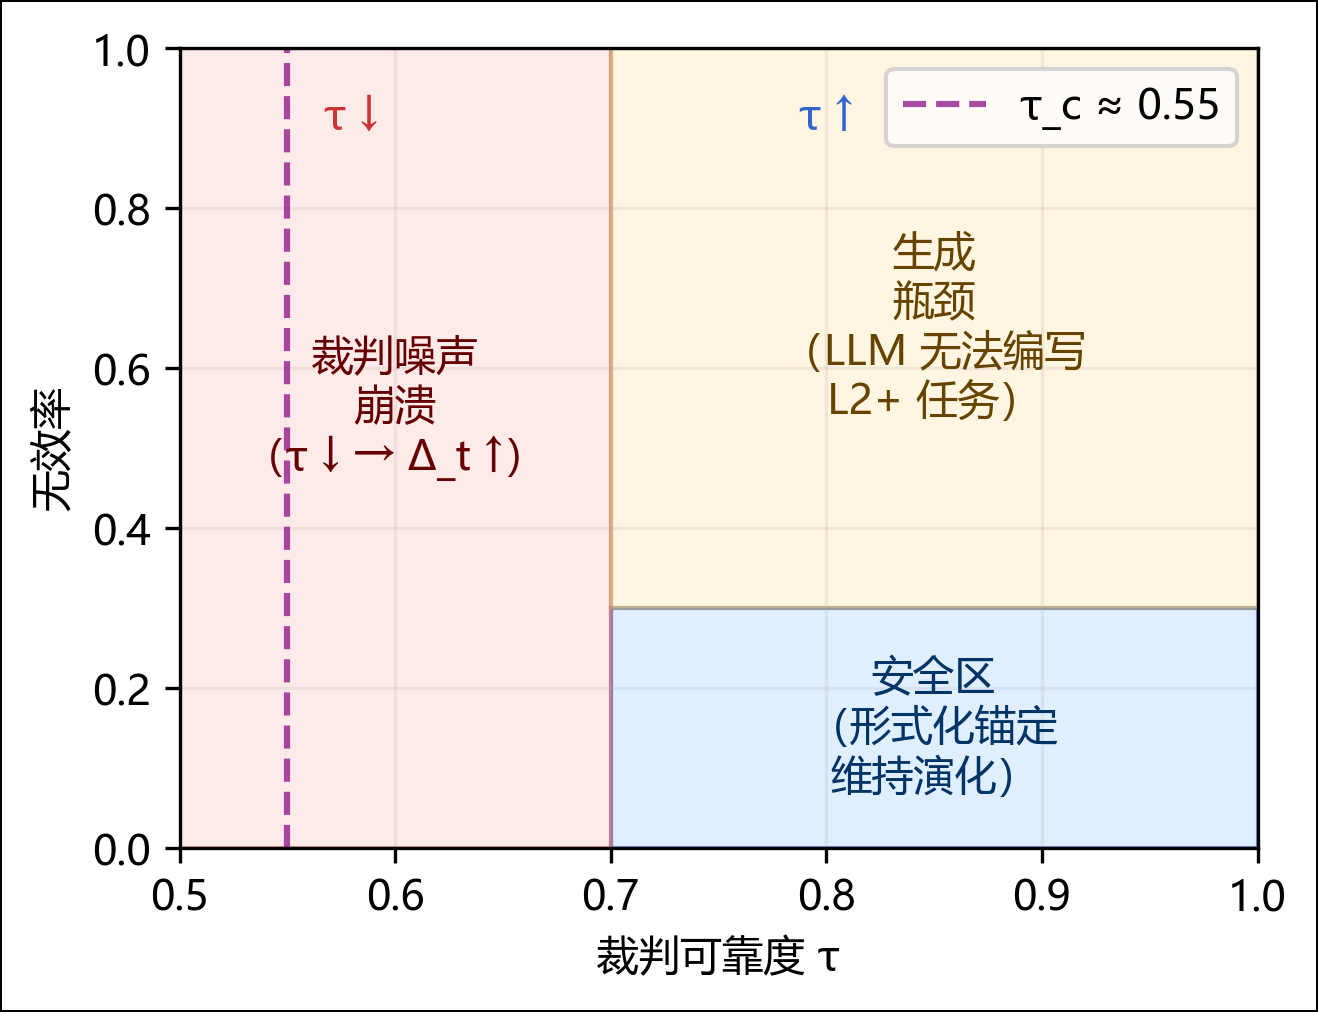
\includegraphics[width=\linewidth]{figures_zh/fig1_dual_bottleneck.png}
  \end{minipage}\hfill
  \begin{minipage}{0.48\linewidth}
    \centering
    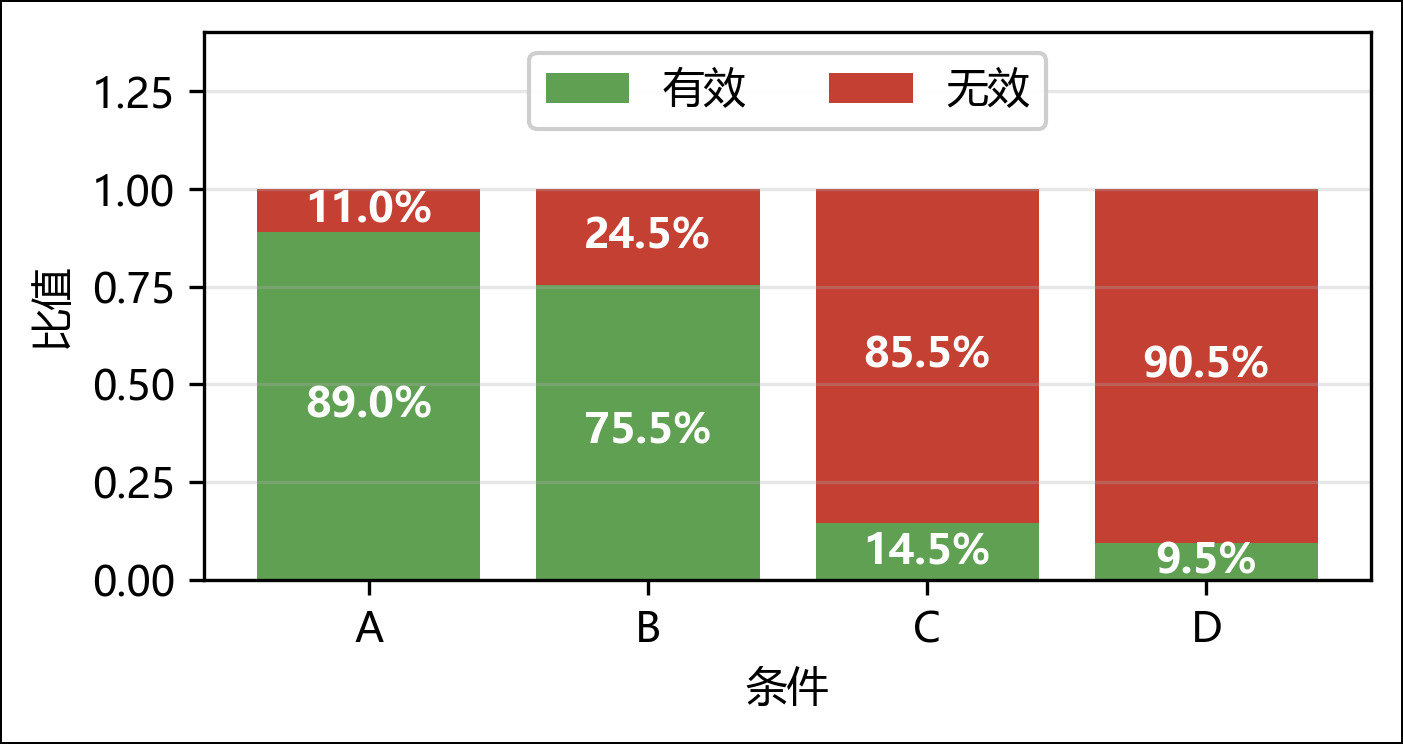
\includegraphics[width=\linewidth]{figures_zh/fig3_validity_rate.png}
  \end{minipage}
  \caption{左图：安全区即裁判可靠度
  $\tau \ge \tau_c$ 与生成器无效任务率 $\le 0.5$ 的交集。右图：有效任务
  率从 89.0\%（A）和 75.5\%（B）跌至 14.5\%（C）和 9.5\%（D）。}
  \label{fig:bottleneck_and_validity}
\end{figure}

\subsection{两个瓶颈}

在 valid-only 口径下，条件 A（LLM 自评分）给出 $\Delta_t = 0.150$，条件 B
（Z3 锚定）给出 $0.000$：只要任务是良构的，锚定的裁决 \textit{就是}真值，
因此自评分偏离在构造上即消失。在 global 口径下，同样的条件读作
A = 0.243、B = 0.245，因为 B 的 147 个无效轮被计入 $\Delta_t = 1.0$。这是
口径差异，而非数据不一致；见附录~\ref{app:data_consistency} 与
图~\ref{fig:bottleneck_and_validity}。

裁判并不是唯一的瓶颈。一旦启用种群博弈（C 与 D），控制器
会把任务推向 L2/L3，而教师无法可靠地编写位向量与数组约束：
有效率从 89.0\%（A）和 75.5\%（B）跌至 14.5\%（C）和 9.5\%（D）。这些失败
\textit{并非}按难度分级——它们聚集在过渡处，因为控制器一直把难度维持在
高位，而教师持续失败。称之为\textbf{伪难度陷阱}：
系统自以为在解决更难的问题，实际上却把预算花在了永远无法进入
验证环节的任务上。学生并没有过错；每一个含有有效任务的轮都被正确解决
（图~\ref{fig:bottleneck_and_validity}）。

\subsection{预算分解}

因此，这两个瓶颈\textbf{共享同一份预算}。给定可容忍的 global 误差
$\Delta_t^{\max}$，留给裁判噪声的额度为

\[
  \Delta_{\mathrm{judge}}^{\mathrm{budget}} = 1 - \frac{1-\Delta_t^{\max}}{1-\Delta_t^{\mathrm{gen}}}
  \qquad\Longrightarrow\qquad
  \tau_c = \sqrt{1 - 2\,\Delta_{\mathrm{judge}}^{\mathrm{budget}}}
\]

因此，$\tau_c$ 并不是某个条件的机制所固有的属性——它是
\textbf{推导}出来的，取决于生成器瓶颈在预算中剩下多少。一个
$\Delta_t^{\mathrm{gen}}$ 较大的条件，在相同的总容忍度下需要更可靠的裁判，但真正的驱动因素是
预算的分配，而不是 $\tau_c$ 本身。

具体地，在 $\Delta_t^{\max} = 0.60$ 时：条件 B（$\Delta_t^{\mathrm{gen}} = 0.245$）需要
$\tau_c \approx 0.24$，而 C 与 D（$\Delta_t^{\mathrm{gen}} = 0.855$ 和 $0.905$）在
\textbf{任何}裁判可靠度下都无法满足该预算，因为它们的生成器瓶颈本身就已超出
预算。这才是预算直觉的正确形式，它把双重瓶颈框架从一种
诊断转变为一条核算规则。

% ===========================================================================
% 5. 裁判可靠度阈值
% ===========================================================================
\section{裁判可靠度阈值}
\label{sec:judge}

本节只问一个问题：给定一个能够产生候选改进的生成器，裁判必须多可靠，迭代式自我改进才能带来净收益？分四步回答。\S\ref{sec:noise} 定义了把裁判可靠度参数化的噪声注入协议。\S\ref{sec:empirical_tau} 在真实智能体轨迹上估计经验阈值 $\tau_c$。\S\ref{sec:analytical} 从合成律出发推导 $\tau_c$ 的闭式表达式。\S\ref{sec:theorem1} 陈述并证明由此得到的可靠度定理。

\subsection{噪声注入协议}
\label{sec:noise}

通过对每个裁决以概率 $p = (1-\tau)/2$ 进行翻转来建模不可靠的裁判，
对 SAT 与 UNSAT 对称处理。每一轮有两个独立的 Z3 调用被注入噪声——
即对教师任务的裁决和对学生答案的裁决——因此它们独立地翻转。

\subsection{经验 $\tau_c$}
\label{sec:empirical_tau}

在条件 B 与 D 上把 $\tau$ 扫过八个取值 $\{0.55, 0.60, 0.65, 0.70, 0.75, 0.80, 0.90, 1.00\}$，
每个格子（cell）50 轮（共 800 轮），使用 \textbf{真实的} DeepSeek V4
Flash API。所有轮都被固定在难度 L1，以使生成器一侧的瓶颈保持
不变，只有裁判的可靠度发生变化。经验曲线见附录~A，
图~\ref{fig:tau_c_curve_appendix}。

一次先导性估计曾给出 $\tau_c(D) = 0.90$ 与 $\tau_c(B) = 0.55$。
该差距在 L1 隔离下未能复现：固定难度恰好移除了该假设所诉诸的机制。

在八个被扫描的 $\tau$ 取值上，条件 B 实测的逐格子均值 $\Delta_t$ 从
$\tau = 0.55$ 时的 0.30 下降到 $\tau = 1.00$ 时的 0.00。其形状是开口
向下的抛物线，而非直线，并且它在 $\tau = 0$ 处穿过 0.5，而不是穿过 1.0。这两个
特征最终都被证明对该机制具有诊断意义，如第~5.3~节所示。检测到的阈值为
在所有三种口径（combined、$\Delta_t$、correct-rate）下 $\tau_c(B) = \tau_c(D) = 0.55$。

\subsection{解析公式}
\label{sec:analytical}

\textbf{假设 1（裁判噪声）。} 每个 Z3 裁决都被独立翻转，其概率为

\[
  p = \frac{1-\tau}{2}
\]

\textbf{假设 2（每轮两次独立判定）。} 一轮涉及两次彼此独立的 Z3 调用：
一次产出对教师任务的裁决（该结果成为 \texttt{expected}），另一次产出
对学生答案的裁决。它们是彼此分离的进程，并且独立地翻转。

当且仅当两个裁决\textbf{一致}时——即都未被翻转，或都被
翻转时——该轮才被记为正确：

\[
  P(\text{correct}) = (1-p)^2 + p^2
\]

代入 $p = (1-\tau)/2$，从而 $1-p = (1+\tau)/2$：

\[
  P(\text{correct}) = \left(\frac{1+\tau}{2}\right)^2 + \left(\frac{1-\tau}{2}\right)^2
  = \frac{(1+\tau)^2 + (1-\tau)^2}{4} = \frac{2 + 2\tau^2}{4} = \frac{1+\tau^2}{2}
\]

因此

\[
  \boxed{\;\Delta_t(\tau) = 1 - P(\text{correct}) = \frac{1-\tau^2}{2}\;}
\]

\textbf{$\tau^2$ 与 $1/2$ 从何而来。} $\tau^2$ 是两个一致项之和——
都正确贡献 $((1+\tau)/2)^2$，都被翻转贡献 $((1-\tau)/2)^2$——
它们的交叉项相互抵消，剩下 $(1+\tau^2)/2$；因此该指数是每轮独立
判定的次数，而不是裁判自身的属性。$1/2$ 来自 SAT/UNSAT 的二元对称性：在
$\tau = 0$ 时，两个独立的随机裁决有一半的时间一致，这就是曲线左端为何锚定在
0.5 而不是 1.0。

在八个被扫描的 $\tau$ 取值上，实测的逐格子均值与闭式解吻合，具体为

\begin{itemize}
  \item MAE = \textbf{0.0258}，RMSE = 0.0329（条件 B）
  \item MAE = \textbf{0.0520}，RMSE = 0.0660（条件 D）
\end{itemize}

\textbf{一个具有判别力的检验。} 假设 2 中的机制并不是唯一能给出
相同 $\Delta_t(\tau)$ 的解释。另一种解释——裁判以概率 $\tau$ 判断正确
\textit{且}系统以概率 $\tau$ 接受该判断——预测
$P(\text{correct}) = \tau^2$，而非 $(1+\tau^2)/2$。两者差异悬殊，因此实测的
\texttt{correct\_rate} 无需任何拟合即可区分它们：

\begin{center}
\small
\begin{tabular}{@{}llr@{}}
  \toprule
  模型 & $P(\text{correct})$ & 相对实测 \texttt{correct\_rate} 的 MAE \\
  \midrule
  两次独立判定（\textbf{本工作}） & $(1 + \tau^2)/2$ & \textbf{0.0389} \\
  裁判 + 接受 & $\tau^2$ & 0.2291 \\
  \bottomrule
\end{tabular}
\end{center}

在 16 个 $(\tau, \text{condition})$ 格子中，两次判定模型在 13 个上更接近、在 2 个上持平，
在 1 个上落败。在 $\tau = 0.80$ / 条件 B 处，它预测 0.8200，而实测为 0.8200。
接受假说在 MAE 上以六倍的差距被拒绝。

\textbf{反解模型。} 由 $\Delta_t = (1 - \tau^2)/2$ 解出 $\tau$，得到设计规则

\[
  \tau_c = \sqrt{1 - 2\,\Delta_t^{\max}}
\]

因此，一个能够容忍误差下界 $\Delta_t^{\max}$ 的系统，需要可靠度至少达到该值的
裁判：

\begin{center}
\small
\begin{tabular}{@{}rr@{}}
  \toprule
  $\Delta_t$ 预算 & 所需的 $\tau_c$ \\
  \midrule
  0.05 & 0.949 \\
  0.10 & 0.894 \\
  0.15 & 0.837 \\
  0.20 & 0.775 \\
  0.25 & 0.707 \\
  \bottomrule
\end{tabular}
\end{center}

这是该结果在实践中有用的形式：它把对评估误差的容忍度转换为
对裁判的最低可靠度要求，而无需重新运行扫描。请注意
可达性上界——没有任何裁判可靠度能把 $\Delta_t$ 保持在 0.5 以下，因为 $\Delta_t(0) = 1/2$。
解析拟合已叠加显示在附录~A、图~\ref{fig:analytical_fit_appendix} 中。

\subsection{定理 1：裁判可靠度阈值}
\label{sec:theorem1}

在第~5.3~节所述的假设下，以定理的形式陈述该阈值。
图~\ref{fig:theorem1} 展示了该阈值。

\textbf{定理 1。} \textit{系统的期望评估偏差为}

\[
  \Delta_t(\tau) \;=\; \frac{1-\tau^{2}}{2}
\]

\textit{不含自由参数；等价地，$P(\text{correct}) = (1+\tau^{2})/2$，且
$\Delta_t(0) = 1/2$。}

\textbf{逆向（设计）形式。} 解出 $\tau$ 可得在可容忍偏差 $\Delta_t^{\max}$ 下
最小的可接受裁判可靠度：

\[
  \tau_c \;=\; \sqrt{1 - 2\,\Delta_t^{\max}}
\]

由于 $\Delta_t(0) = 1/2$，没有任何裁判可靠度能把偏差保持在 $1/2$ 以下，因此该规则
仅在 $\Delta_t^{\max} \in [0, 1/2)$ 上有定义。

\textbf{推论（裁判稀缺性）。} $\tau_c$ 是可容忍偏差的函数，\textbf{而}不是
系统的常数。在 $\Delta_t^{\max} = 0.35$ 时，一个大约每五次裁决错一次的裁判
（$\tau \approx 0.55$）仍能使系统保持在安全区内；把容忍度收紧到
$0.05$ 则需要 $\tau \approx 0.95$。

\textbf{经验验证。} 在 800 个真实 API 轮上拟合（8 个 $\tau$ 取值 $\times$ 2
个条件 $\times$ 50 轮，难度固定为 L1）：MAE = \textbf{0.0258} / RMSE = 0.0329（B）
以及 MAE = \textbf{0.0520} / RMSE = 0.0660（D）。

\textbf{注记（被拒绝的替代模型）。} 一个竞争模型——裁判以概率 $\tau$ 判断正确
\textit{且}系统以概率 $\tau$ 接受该判断——预测
$P(\text{correct}) = \tau^{2}$，因而 $\Delta_t = 1-\tau^{2}$。判别检验\textbf{无需任何拟合}
即可拒绝它：相对于实测 \texttt{correct\_rate} 的 MAE 为 0.2291，而
定理 1 为 0.0389；在 16 个格子中定理 1 于 13 个上更接近、2 个持平、1 个落败。在
$\tau = 0.55$ 处，它预测 0.6975，而实测为 0.3000（B）和 0.3200（D）。本文没有任何结果
使用 $\Delta_t = 1-\tau^{2}$。

\textbf{与 Ratchet 界的关系。} Ratchet 的分析给出 $(1 - \tau)/2$，作为
\textbf{单次}判定被翻转的概率。量是\textbf{双次}判定
系统的稳态误差。两者通过一致概率相联系，而这种
区别是结构性的，而非数值上的：

\begin{center}
\small
\begin{tabular}{@{}lll@{}}
  \toprule
  设定 & 每次决策中的噪声事件 & 误差 \\
  \midrule
  技能消除（Ratchet） & 一次判定，然后据此行动 & $(1 - \tau)/2$ \\
  答案评估（本工作） & 裁判的裁决\textbf{与}系统的裁决必须一致 & $(1 - \tau^2)/2$ \\
  \bottomrule
\end{tabular}
\end{center}

两者之间的映射是两次判定中恰好只有一次被翻转的概率：

\[
  \Delta_t = 2p(1-p) \;\xrightarrow{p \to 0}\; 2p = 1-\tau
\]

因此，在高可靠度极限下两者在一阶上一致，而离开该极限后则以二次方式
分岔。在 $\tau = 0.95$ 时，单次判定界预测 0.025，而双次判定模型
预测 0.049：在该可靠度下，要求两个独立裁决一致会使可容忍误差
减半。Ratchet 的界是系统仅依据一次判定行动时的特例；
此处的公式把它推广到依据两次判定之间的一致性行动的系统。

\begin{figure*}[t]
  \centering
  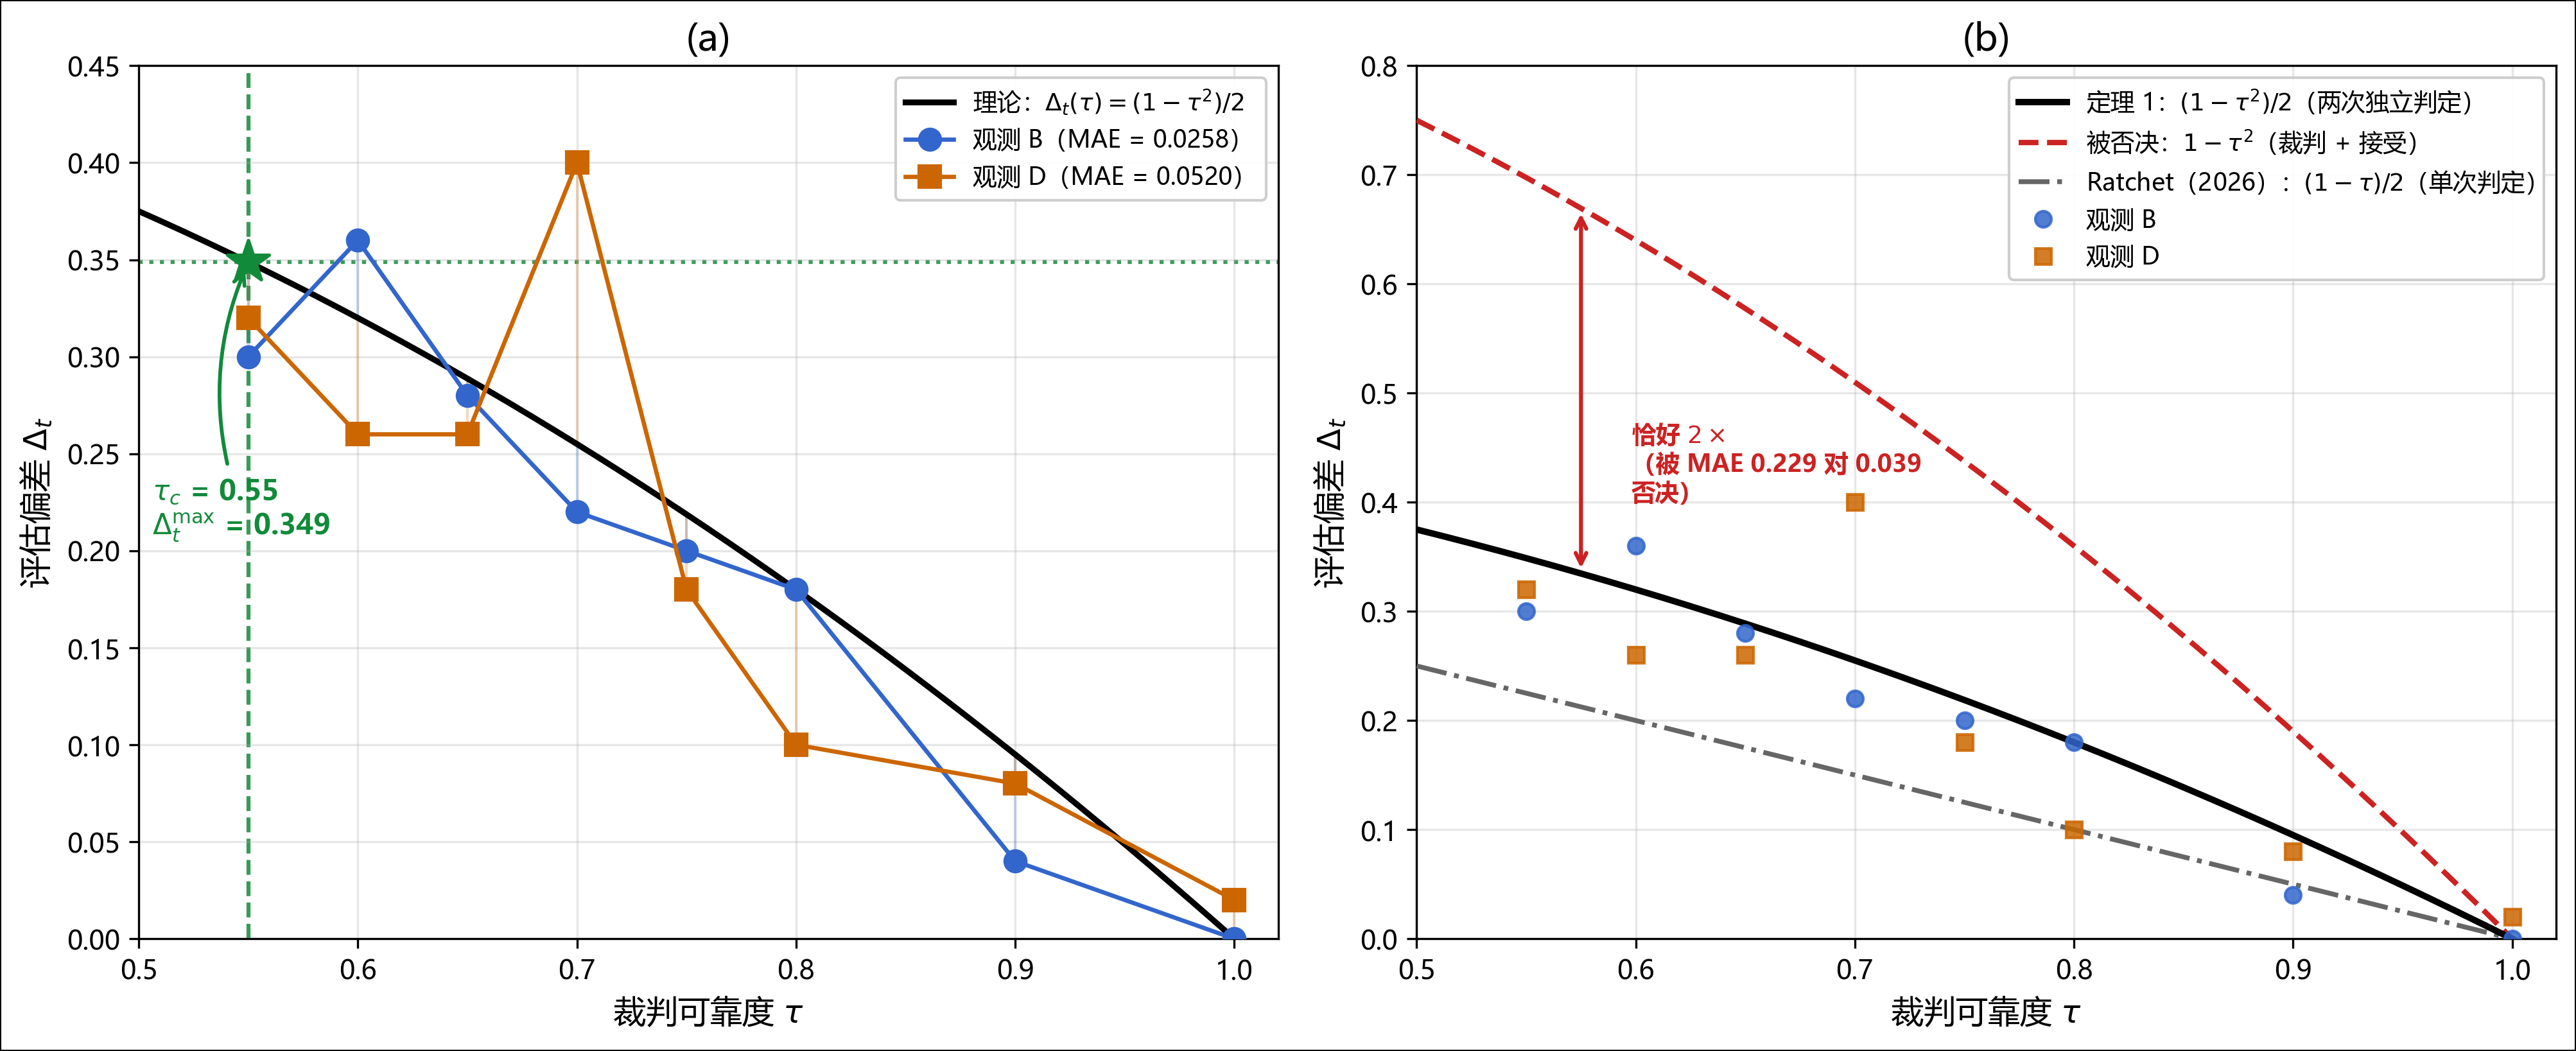
\includegraphics[width=\textwidth]{figures_zh/fig5c_theorem1.png}
  \caption{子图 (a)：闭式解 $\Delta_t(\tau) = (1-\tau^2)/2$ 与条件 B 和 D 的真实 API 扫描
  的对比，其中标出了实测的 $\tau_c = 0.55$ 及相应的
  $\Delta_t^{\max} = 0.349$。子图 (b)：同一闭式解与被拒绝的接受
  模型（$\Delta_t = 1-\tau^2$）以及 Ratchet 的单次判定界（$(1-\tau)/2$）的对比；接受
  模型恰好高出两倍，并被第~5.3~节的判别检验所拒绝。}
  \label{fig:theorem1}
\end{figure*}

% ===========================================================================
% 6. 扩展生成器能力
% ===========================================================================
\section{扩展生成器能力}

第~\ref{sec:judge} 节把裁判可靠度视为绑定约束。现在提出其对偶的问题：一旦可靠的裁判已经可用，是什么限制了生成器\emph{使用}它的能力？首先给出一个四层约束框架（\S\ref{sec:fourlayer}），随后在真实 API 调用上验证它（\S\ref{sec:api}），最后报告能够把真实的生成器改进与裁判侧假象区分开的统计检验（\S\ref{sec:stat}）。

\subsection{四层约束框架}
\label{sec:fourlayer}

第~4.3 节表明，自由形式的代码生成是生成器侧的绑定约束。因此
将其替换为一条四层流水线：

\begin{enumerate}
  \item \textbf{JSON 骨架生成。} 教师提示词要求输出 JSON 对象而非
        Python 代码，从而消除括号匹配与变量声明这两类失败。
  \item \textbf{确定性渲染。} 由模板化渲染器把骨架转换为 Z3 Python
        代码，因此输出在构造上即语法合法。
  \item \textbf{符号反馈。} Z3 错误码被映射为命名补救措施。该映射已实现并有单元测试，
        但实验框架对每个任务只构造一次教师提示词，且传入的是
        \texttt{extra\_constraints=None}，因此提示在下文运行中并未到达模型；
        那些运行真正起作用的是重试预算。
  \item \textbf{课程控制器。} 子档位控制器（连续五轮有效任务率 $> 0.80$ 时提升、
        连续三轮低于 $0.50$ 时降低）已实现并有单元测试
        （\texttt{scripts/difficulty\_controller.py}），但未接入任何一个轮次循环：
        下文的验证把每个等级当作固定因子显式请求。
\end{enumerate}

四层之中，承担下文实测增益的是前两层；后两层已实现并有测试，但并未被这些运行所执行。

\subsection{真实 API 验证}
\label{sec:api}

使用真实的 DeepSeek V4 Flash API，在 240 轮（4 个条件 $\times$ 3 个层级 $\times$ 20 轮）
上验证该约束框架。各条件之间的改进情况见
图~\ref{fig:improvement_comparison}。

在该框架就位后，真实 API 下的有效任务率为 L1 = 100.0\%（80/80）、L2 = 73.8\%
（59/80）、L3 = 83.8\%（67/80）。

在 34 个无效轮次中，33 个是
\texttt{error\_code=1: LLM did not return valid JSON}——模型产出的输出完全无法解析——
另有 1 个是模式违规（不支持的变量类型）。因此，每一个无效轮次都可归因于模型，
而非框架。这是该方法诚实的下限：框架保证良构骨架会变成良构约束集，却无法保证
模型一定产出良构骨架。这也正是为什么上述比率衡量的是生成器能力，
而不是工具链本身的可靠性。

\begin{figure*}[t]
  \centering
  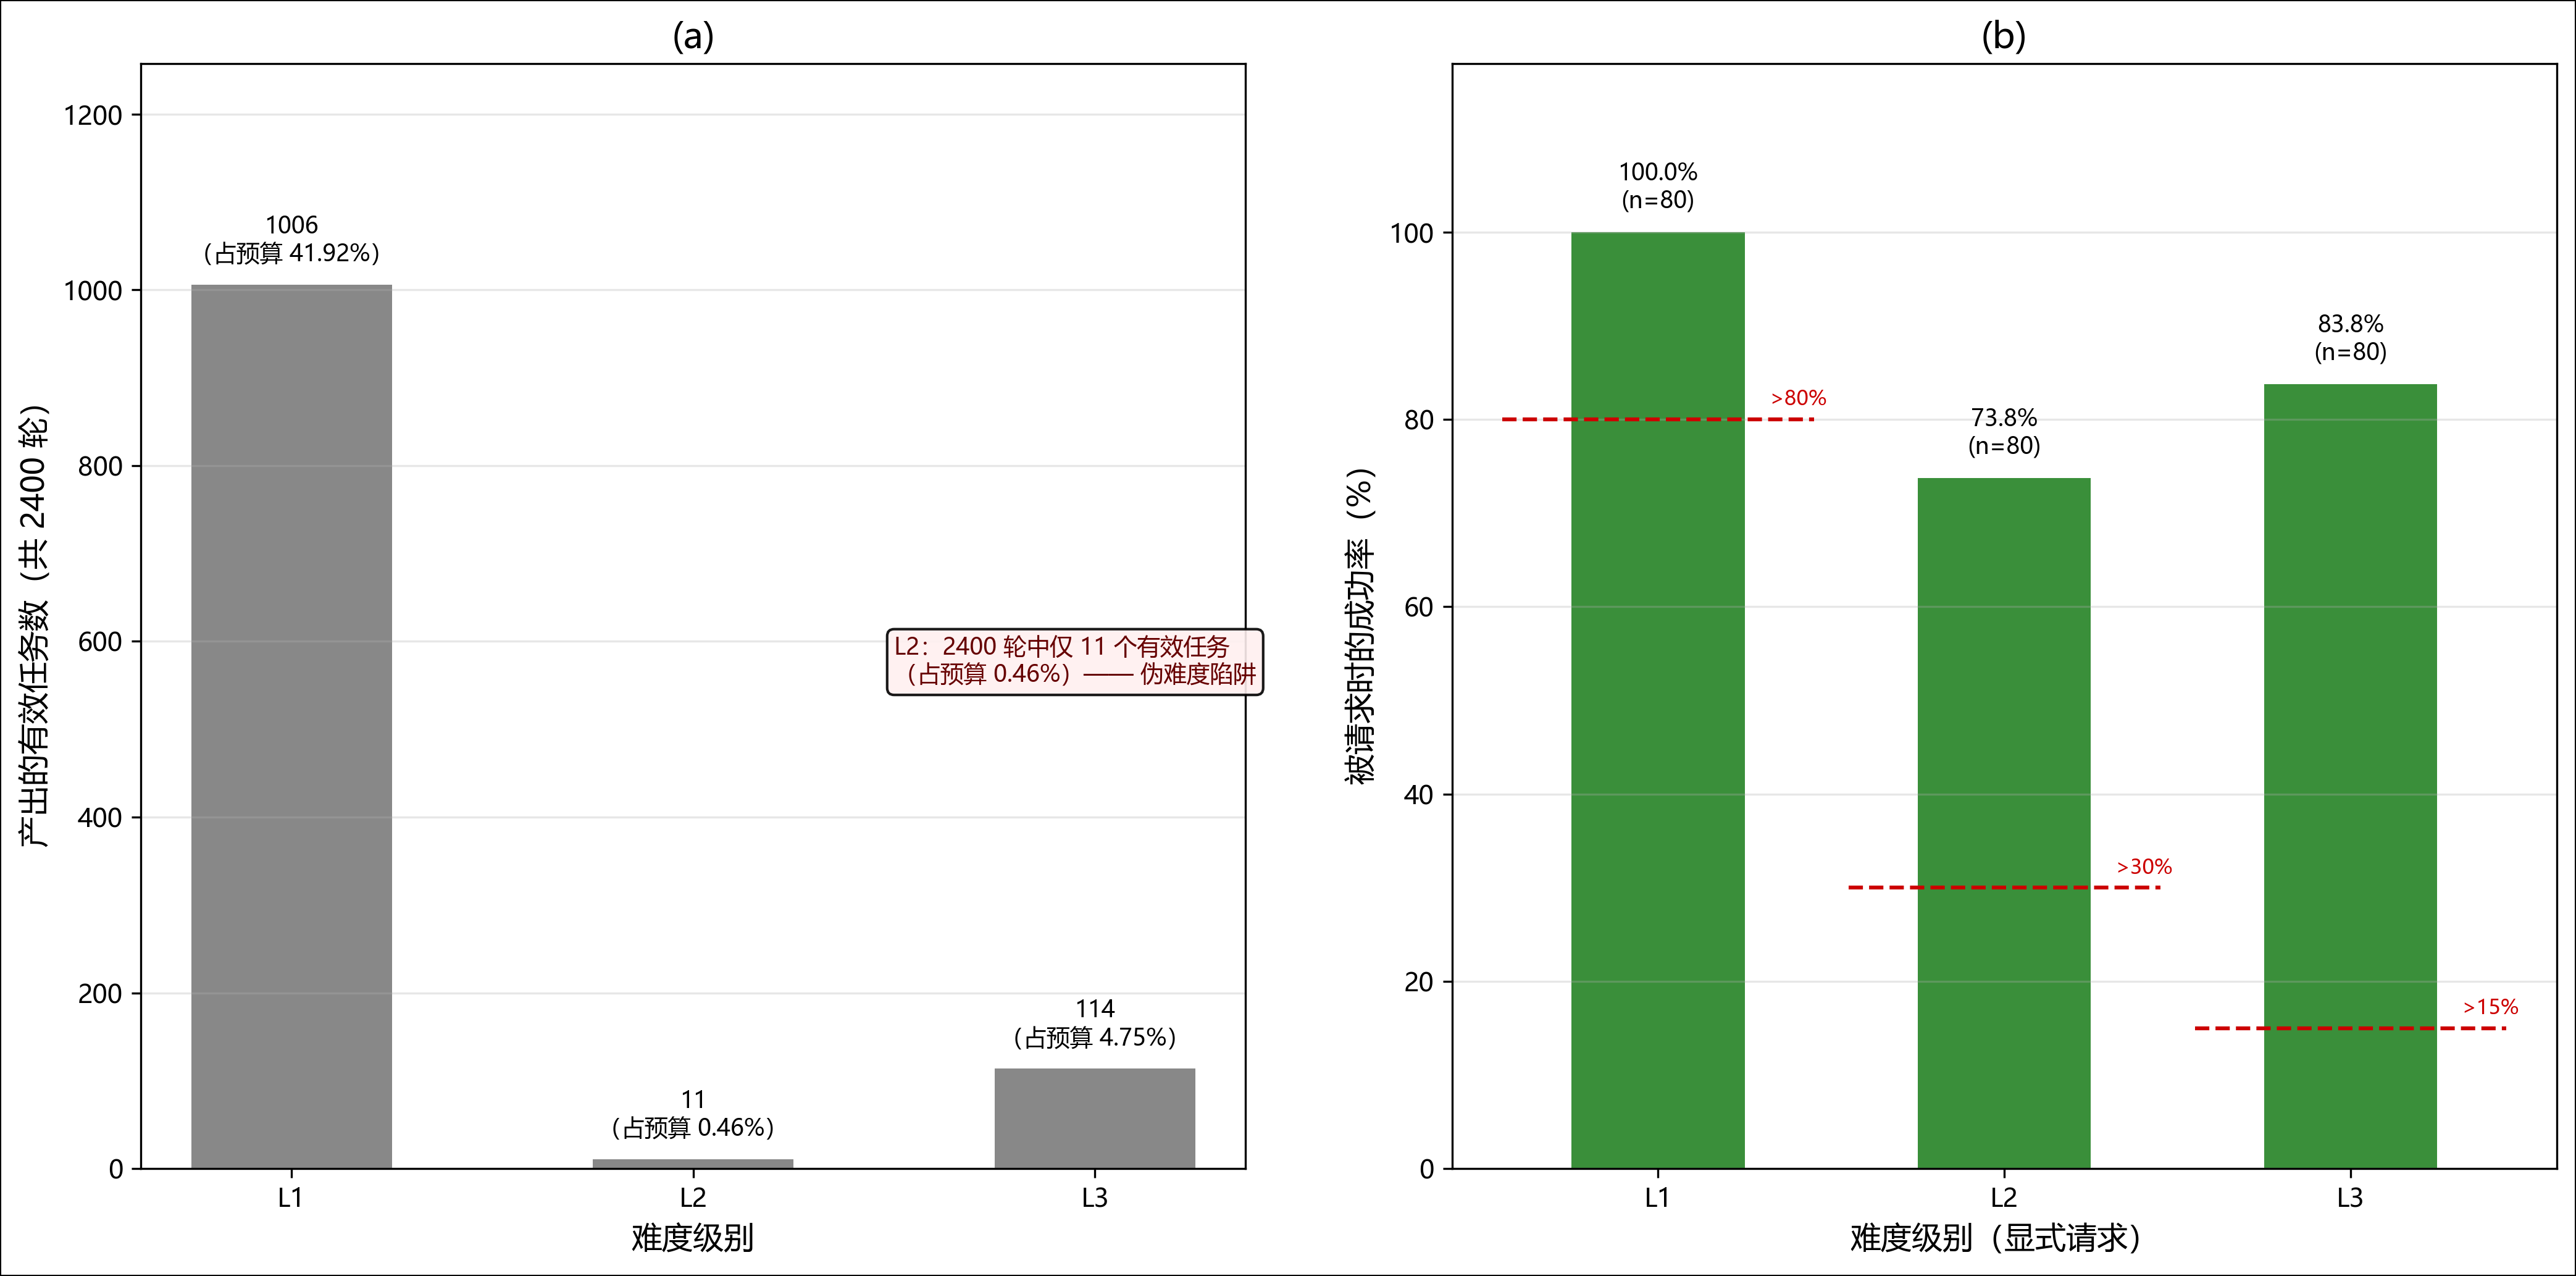
\includegraphics[width=0.7\textwidth]{figures_zh/fig6_improvement_comparison_real.png}
  \caption{在四层约束生成框架启用前/后，真实 API 上的 240 轮
  （4 个条件 $\times$ 3 个层级 $\times$ 20 轮）。采用该框架时的有效任务率为 L1 =
  100.0\%（80/80）、L2 = 73.8\%（59/80）、L3 = 83.8\%（67/80）；而旧版教师
  在 2,400 轮中仅产出 11 个有效 L2 任务与 114 个有效 L3 任务。由于两次运行的预算与
  分母不同，此处比较的是能力，而非比率。}
  \label{fig:improvement_comparison}
\end{figure*}

\subsection{统计验证}
\label{sec:stat}

\S\ref{sec:api} 中的 API 结果显示该框架提升了有效任务率，但这些结果
并未排除一种裁判侧假象：一个更干净的裁判可以提高测量到的有效性，
而生成器质量并无任何真实增益。因此，对已发布的真实 API 日志
施加 Welch 的 $t$ 检验，且不采用任何重采样流程。

\paragraph{逐条件检验。} 60 个框架轮次对 600 个旧版轮次给出：A 为
$t = 4.26$（$p = 2\times10^{-5}$，$d = 0.60$），B 为 $t = 0.82$（$p = 0.41$，$d = 0.11$）。
A 有可测量的改进，而 B 仍为零结果，这与"该框架绑定的是生成器而非裁判"相一致。
而在生成器瓶颈确实绑定的
地方，位移是决定性的：C 从 $\Delta_t = 0.8767$ 变为 $0.1500$（$t = 15.12$，$d = 2.38$），D 从 $0.9050$
变为 $0.1333$（$t = 16.83$，$d = 2.59$）。

\paragraph{口径一致的 L1 检验。} 旧版分母排除了失败轮次，因此只有 L1
可比。在该层级上，改进后的教师显示出更低的 $\Delta_t$（$0.000$ 对 $0.082$；Welch
$t = 34.61$，$p < 10^{-15}$，Cohen's $d = 1.13$，大效应量）。

\paragraph{口径注意事项。} \S\ref{sec:calibers} 的两种口径仅在对无效轮次的处理上
不同：global 口径对每个无效轮次计入 $\Delta_t = 1.0$，valid-only 口径则将其
排除。逐条件检验采用 global 口径——这是保守的选择，因为减少
无效轮次正是该框架所主张的效果。

% ===========================================================================
% 7-8
% ===========================================================================
\section{讨论}

该公式意味着，“足够可靠”并非一种绝对属性。对于一个 $\Delta_t^{\max} = 0.35$ 的
系统，可靠度为 55\% 的裁判即已够用。这重新框定了裁判稀缺问题：实际的
问题不是“能否找到一个完美的裁判？”，而是“在给定生成器
$\Delta_t^{\mathrm{gen}}$ 的前提下，系统能承受多大的容差 $\Delta_t^{\max}$？”

由此导出三项具体的部署前检查（pre-deployment check）。(1) 在控制器被允许
请求的最高难度上测量生成器的误差 $\Delta_t^{\mathrm{gen}}$。若
$\Delta_t^{\mathrm{gen}} \ge \Delta_t^{\max}$，则生成器就是瓶颈；此时改进裁判只是
白费力气。(2) 在一组留出的有效任务上测量裁判的误差；这直接给出 $\tau$。
(3) 将二者代入 $\tau_c = \sqrt{1 - 2\Delta_t^{\max}}$ 并与实测的
$\tau$ 比较。若 $\tau < \tau_c$，预期出现单调漂移；若 $\tau \ge \tau_c$，预期行为
稳定或持续改善。在的情形中，L1 扫描给出 $\tau = \tau_c = 0.55$，而完整的 2,400 轮运行
给出 $\Delta_t^{\mathrm{gen}} = 0.855$（C）与 $0.905$（D），二者均超过 $\Delta_t^{\max} = 0.6$
——这正是伪难度陷阱。

合成律还提示了一个架构方向：自进化系统应把 $\Delta_t^{\mathrm{gen}}$ 与 $\tau$ 作为
一等遥测（telemetry）暴露出来，并以 $\Delta_t^{\mathrm{gen}} < \Delta_t^{\max}$ 作为
难度升级的门控条件。四层约束框架正是其中一种实例
——它降低 $\Delta_t^{\mathrm{gen}}$，直到生成器不再耗尽整份预算，此时
$\tau_c$ 才成为一个有意义的运行阈值。

\section{结论}

着手测量的是：自进化智能体若要改进，裁判必须有多可靠。答案并非
一个固定数值，而是生成器已经花掉多少误差预算的函数：合成律
$1 - \Delta_t^{\mathrm{global}} = (1 - \Delta_t^{\mathrm{gen}})(1 - \Delta_t^{\mathrm{valid}})$
在 2{,}400 个真实 API 轮次上成立至机器精度，并给出一个不含拟合参数的
闭式解 $\tau_c = \sqrt{1 - 2\Delta_t^{\max}}$。由此可得两个结果。第一，伪难度陷阱：
一旦生成器瓶颈超出容差，任何裁判可靠度都无法挽救该循环。第二，
$\tau_c$ 并非系统的常数——一个同时具备种群博弈、蒸馏与圆桌共识的系统，
与一个最小的 Z3 锚定循环返回相同的 $\tau_c$，因为该公式只关心
生成器留下了多少预算。这把自进化问题从“增加更多机制”
重新框定为“先测量预算的分配”。

% ===========================================================================
% REFERENCES
% ===========================================================================
% 用 unsrtnat（而不是 plainnat），使文献编号按首次引用顺序排列：
% 正文中第一次 \cite 会成为 [1]。plainnat 按作者字母序编号，
% 这会让引言开篇处出现 [3]。
\bibliographystyle{unsrtnat}
\bibliography{refs}

% ===========================================================================
% APPENDICES
% ===========================================================================
\appendix

\section{完整图集}

本附录汇集完整图集以供参考。图~\ref{fig:delta_t_global}、\ref{fig:delta_t_L1_phase}、\ref{fig:difficulty_trajectory} 与 \ref{fig:tau_c_gap} 分别展示全局 $\Delta_t$ 轨迹、L1 阶段分解、难度轨迹，以及经验--解析 $\tau_c$ 差距。图~\ref{fig:analytical_fit_appendix}、\ref{fig:validity_by_level_appendix}、\ref{fig:tau_c_curve_appendix} 与 \ref{fig:delta_t_per_round_appendix} 依次补充解析拟合、分级有效任务率、$\tau$ 扫描与逐轮 $\Delta_t$ 分解。

\begin{figure*}[t]
  \centering
  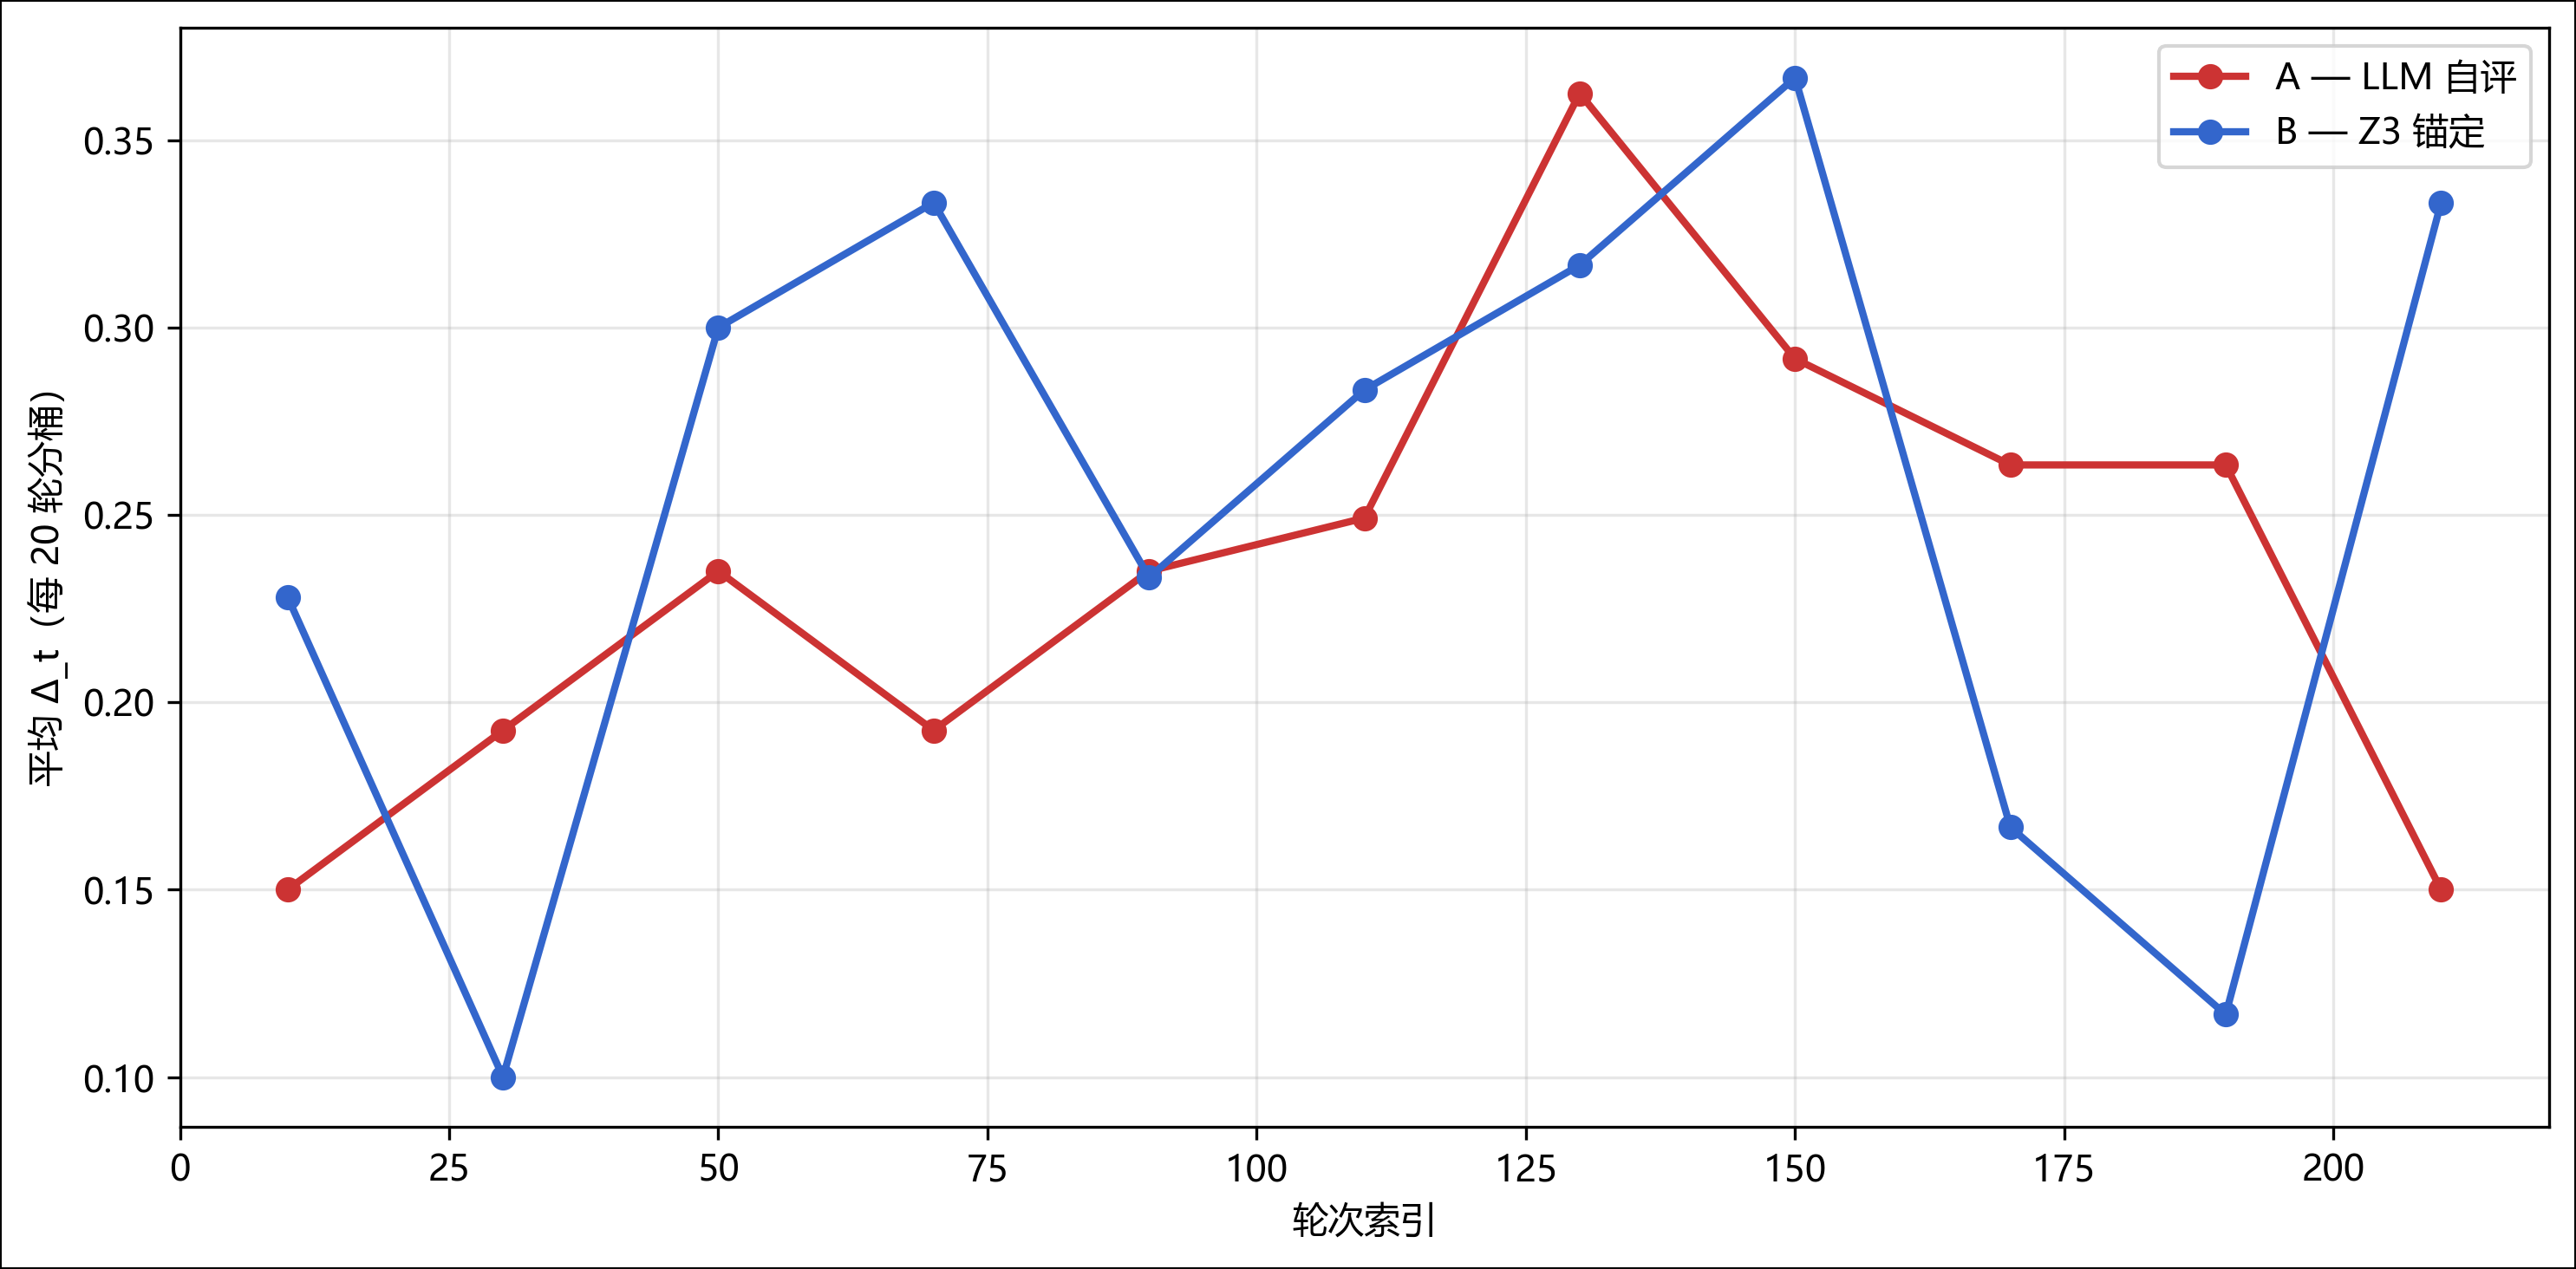
\includegraphics[width=\textwidth]{figures_zh/fig2_delta_t_AB.png}
  \caption{Global 口径的 $\Delta_t$（无效轮次编码为 $\Delta_t=1.0$）。
  条件 A 的平均值为 0.2435，条件 B 的平均值为 0.2450——二者看似
  相近，是因为 B 更高的无效率抵消了其在有效轮次上的零偏差。
  valid-only 口径（图~\ref{fig:delta_t_per_round_appendix}）隔离了裁判
  行为，是比较裁判可靠度时应采用的正确视角。}
  \label{fig:delta_t_global}
\end{figure*}

\begin{figure*}[t]
  \centering
  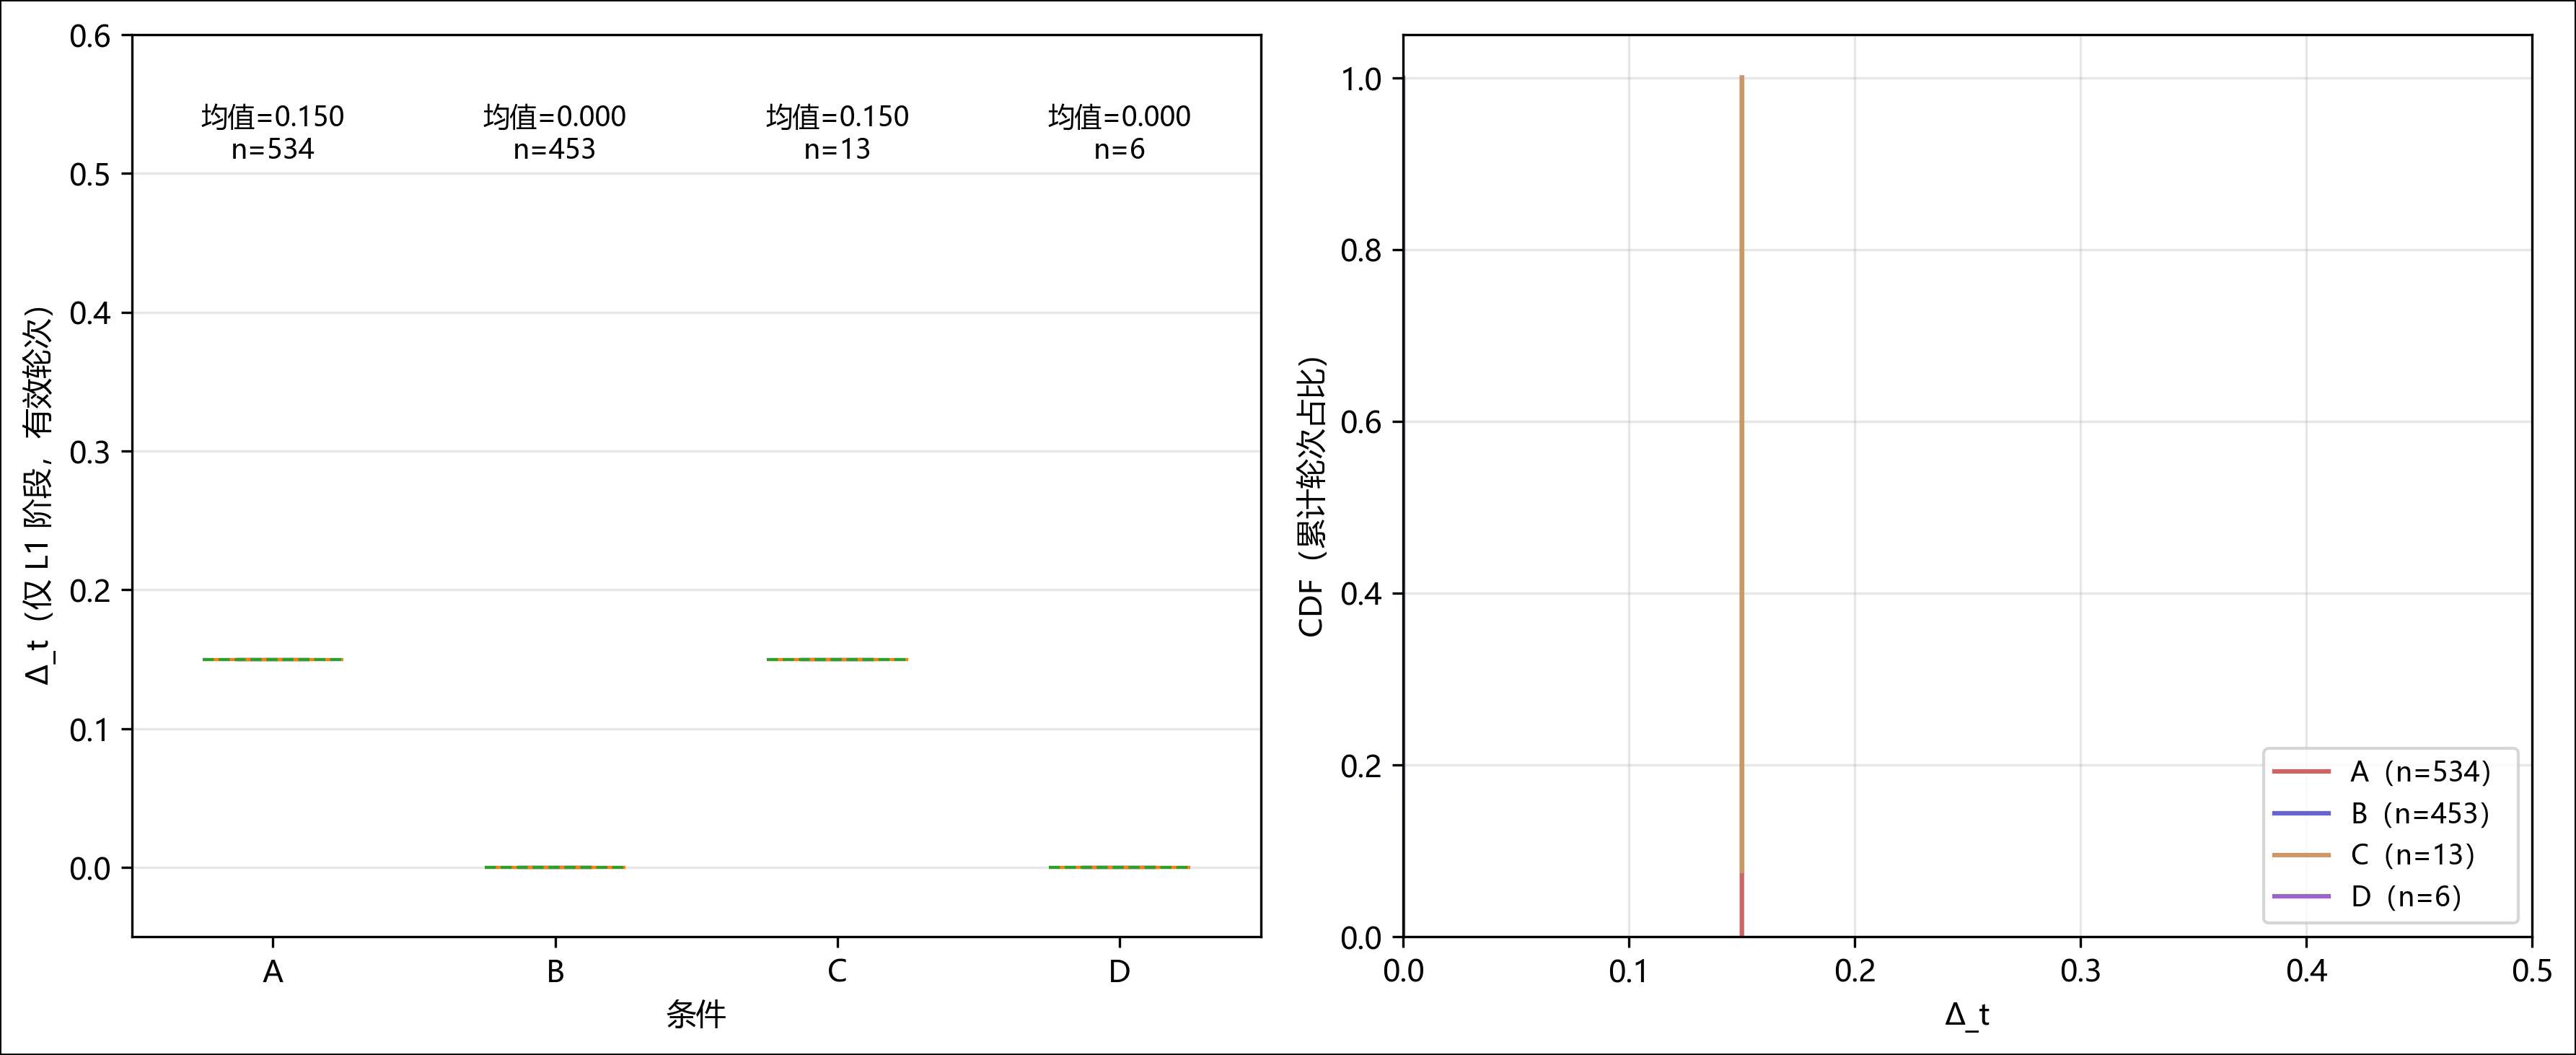
\includegraphics[width=\textwidth]{figures_zh/fig2c_delta_t_L1_only.png}
  \caption{仅限 C/D 被提升到 L2 之前的那些轮次。C/D 在 L1 阶段的 $\Delta_t$
  并\textit{不}比 A/B 更差，因此种群博弈本身并不损害性能——C/D
  后来的退化源自难度升级，而非机制中的缺陷。注意：
  C/D 的 L1 阶段样本量（$n = 13$，$n = 6$）偏小，因为难度控制器
  升级过快。“种群在 L1 上无害”这一断言只是方向性的；更大样本的
  确证留待未来工作。}
  \label{fig:delta_t_L1_phase}
\end{figure*}

\begin{figure*}[t]
  \centering
  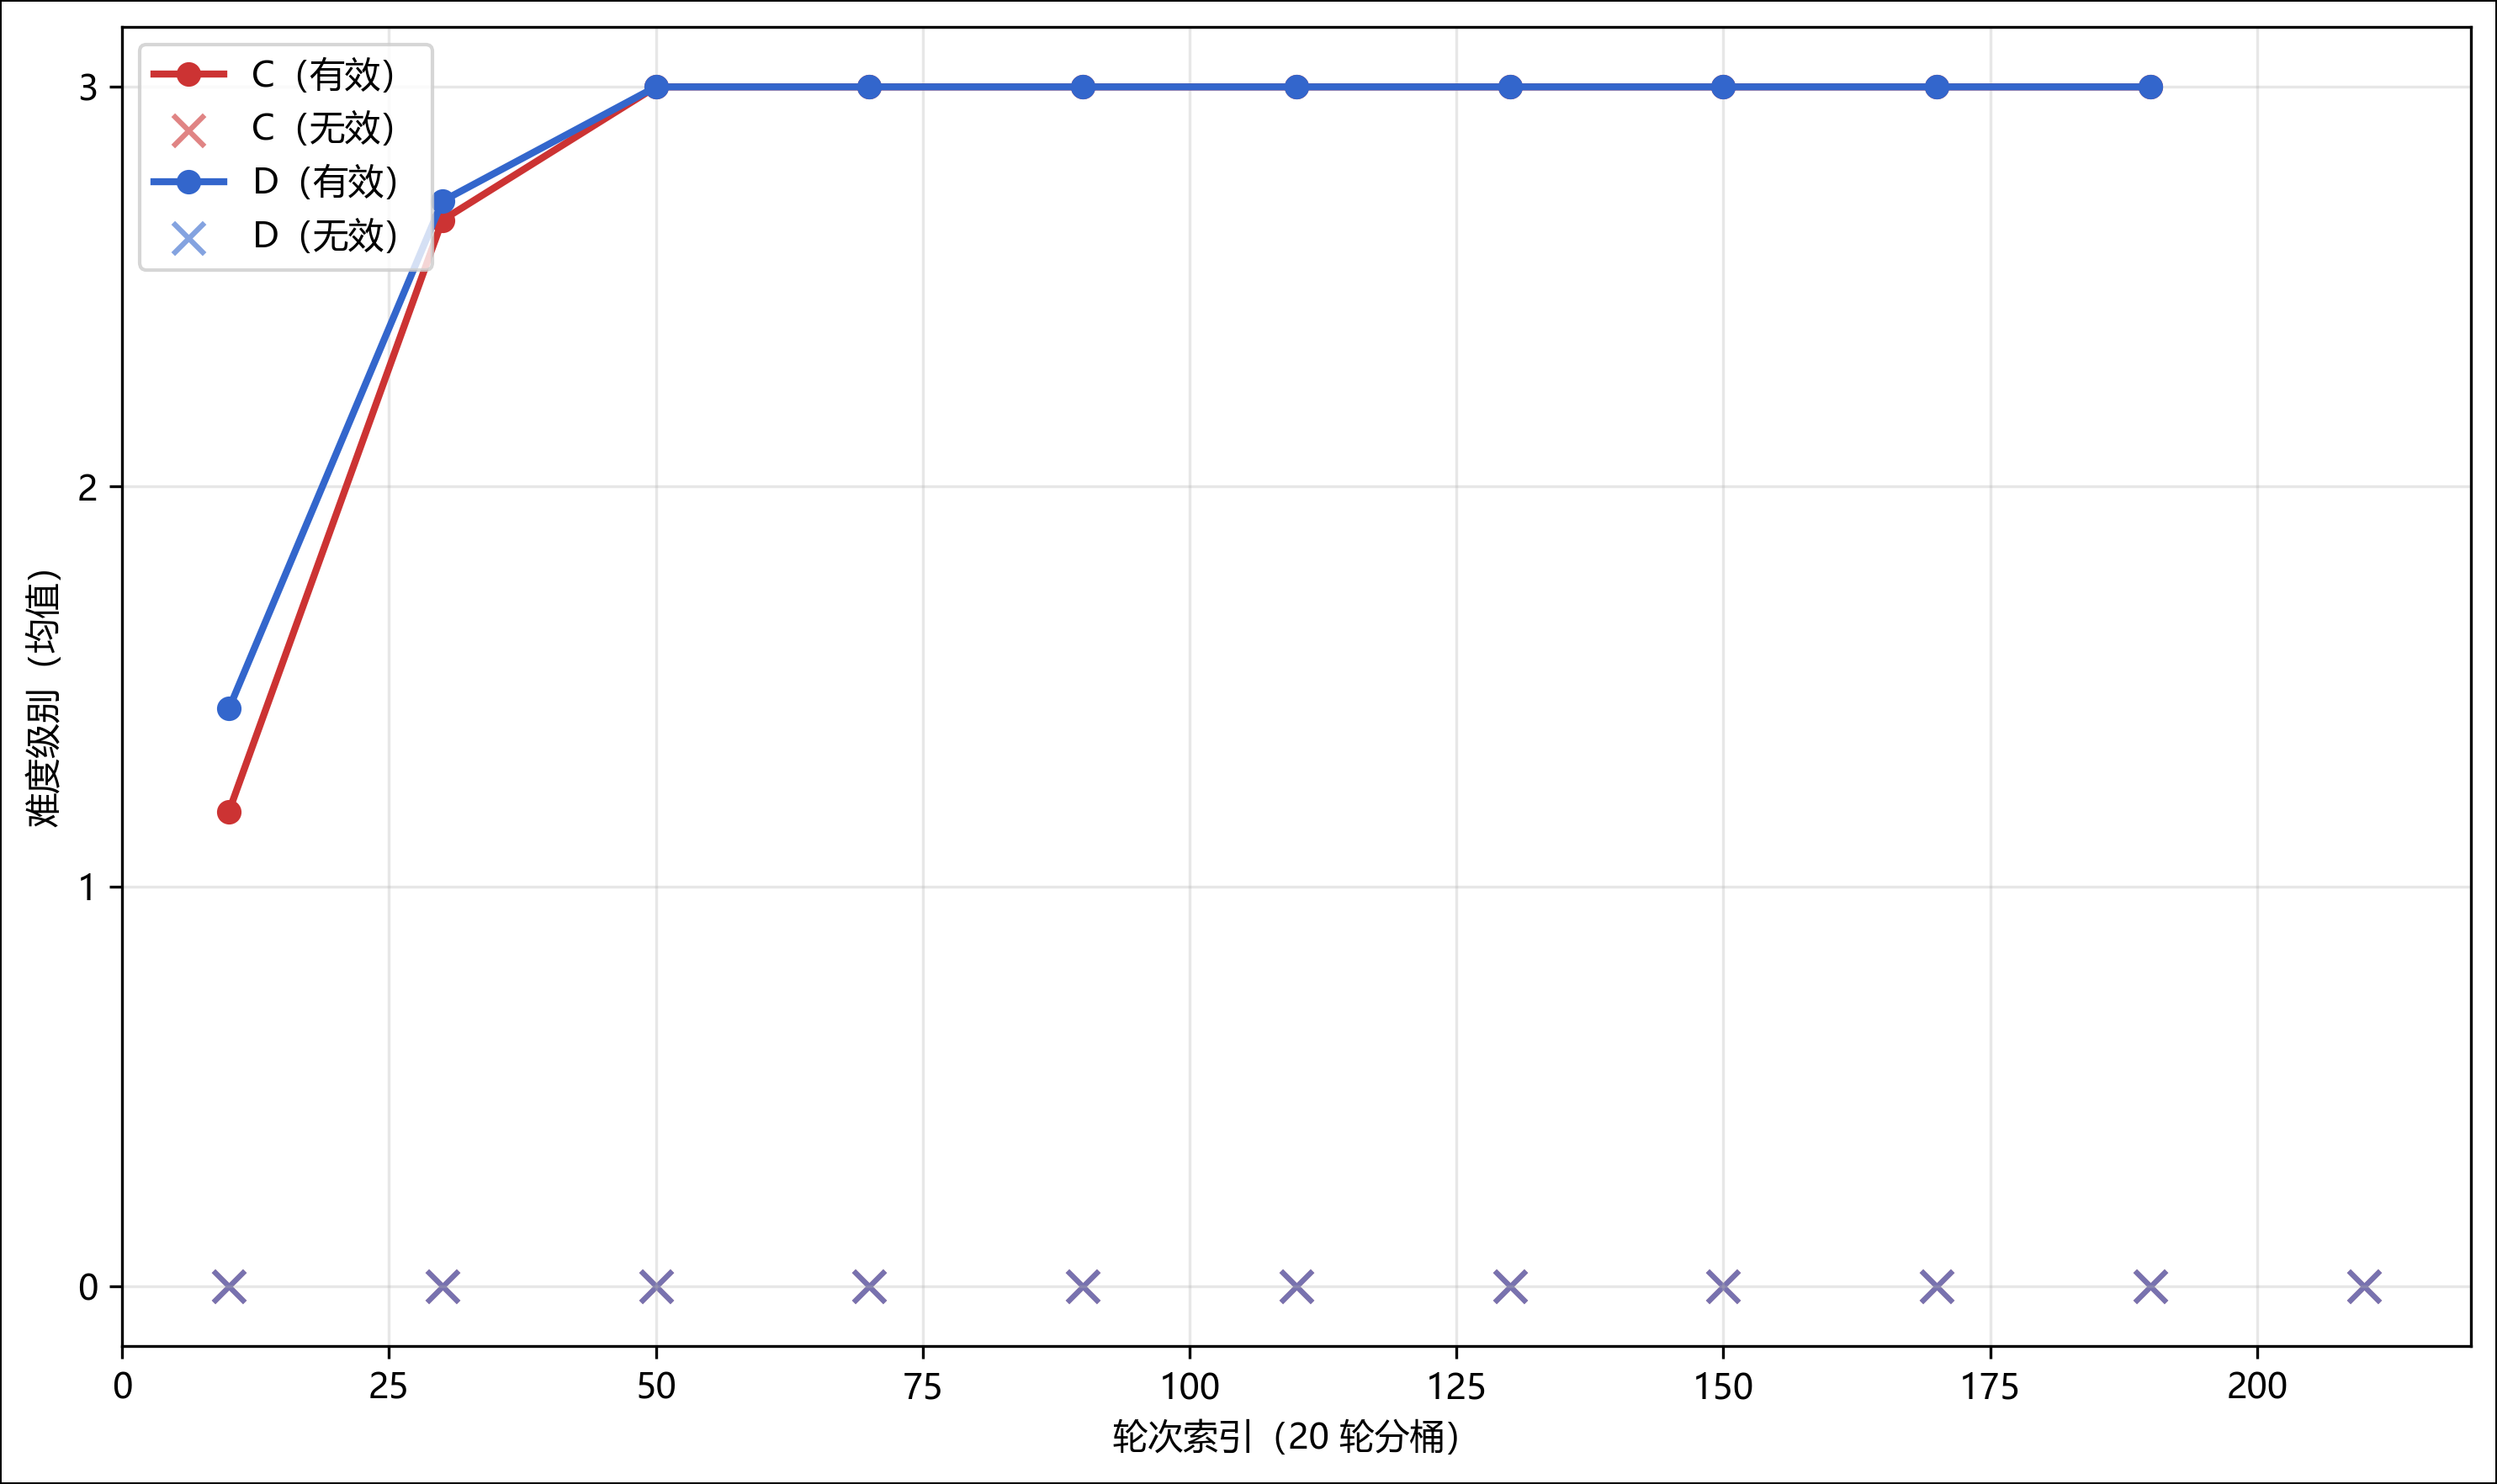
\includegraphics[width=\textwidth]{figures_zh/fig4_difficulty_trajectory.png}
  \caption{条件 C 与 D 的难度轨迹。失败在难度上\textit{并非}均匀
  分布——它们聚集在升级发生的那一刻。一旦层级被提升，
  教师持续失败，而控制器却把层级维持在高位，于是系统自以为
  在解决更难的问题，实际却把预算花在不可用的任务提案上。}
  \label{fig:difficulty_trajectory}
\end{figure*}

\begin{figure*}[t]
  \centering
  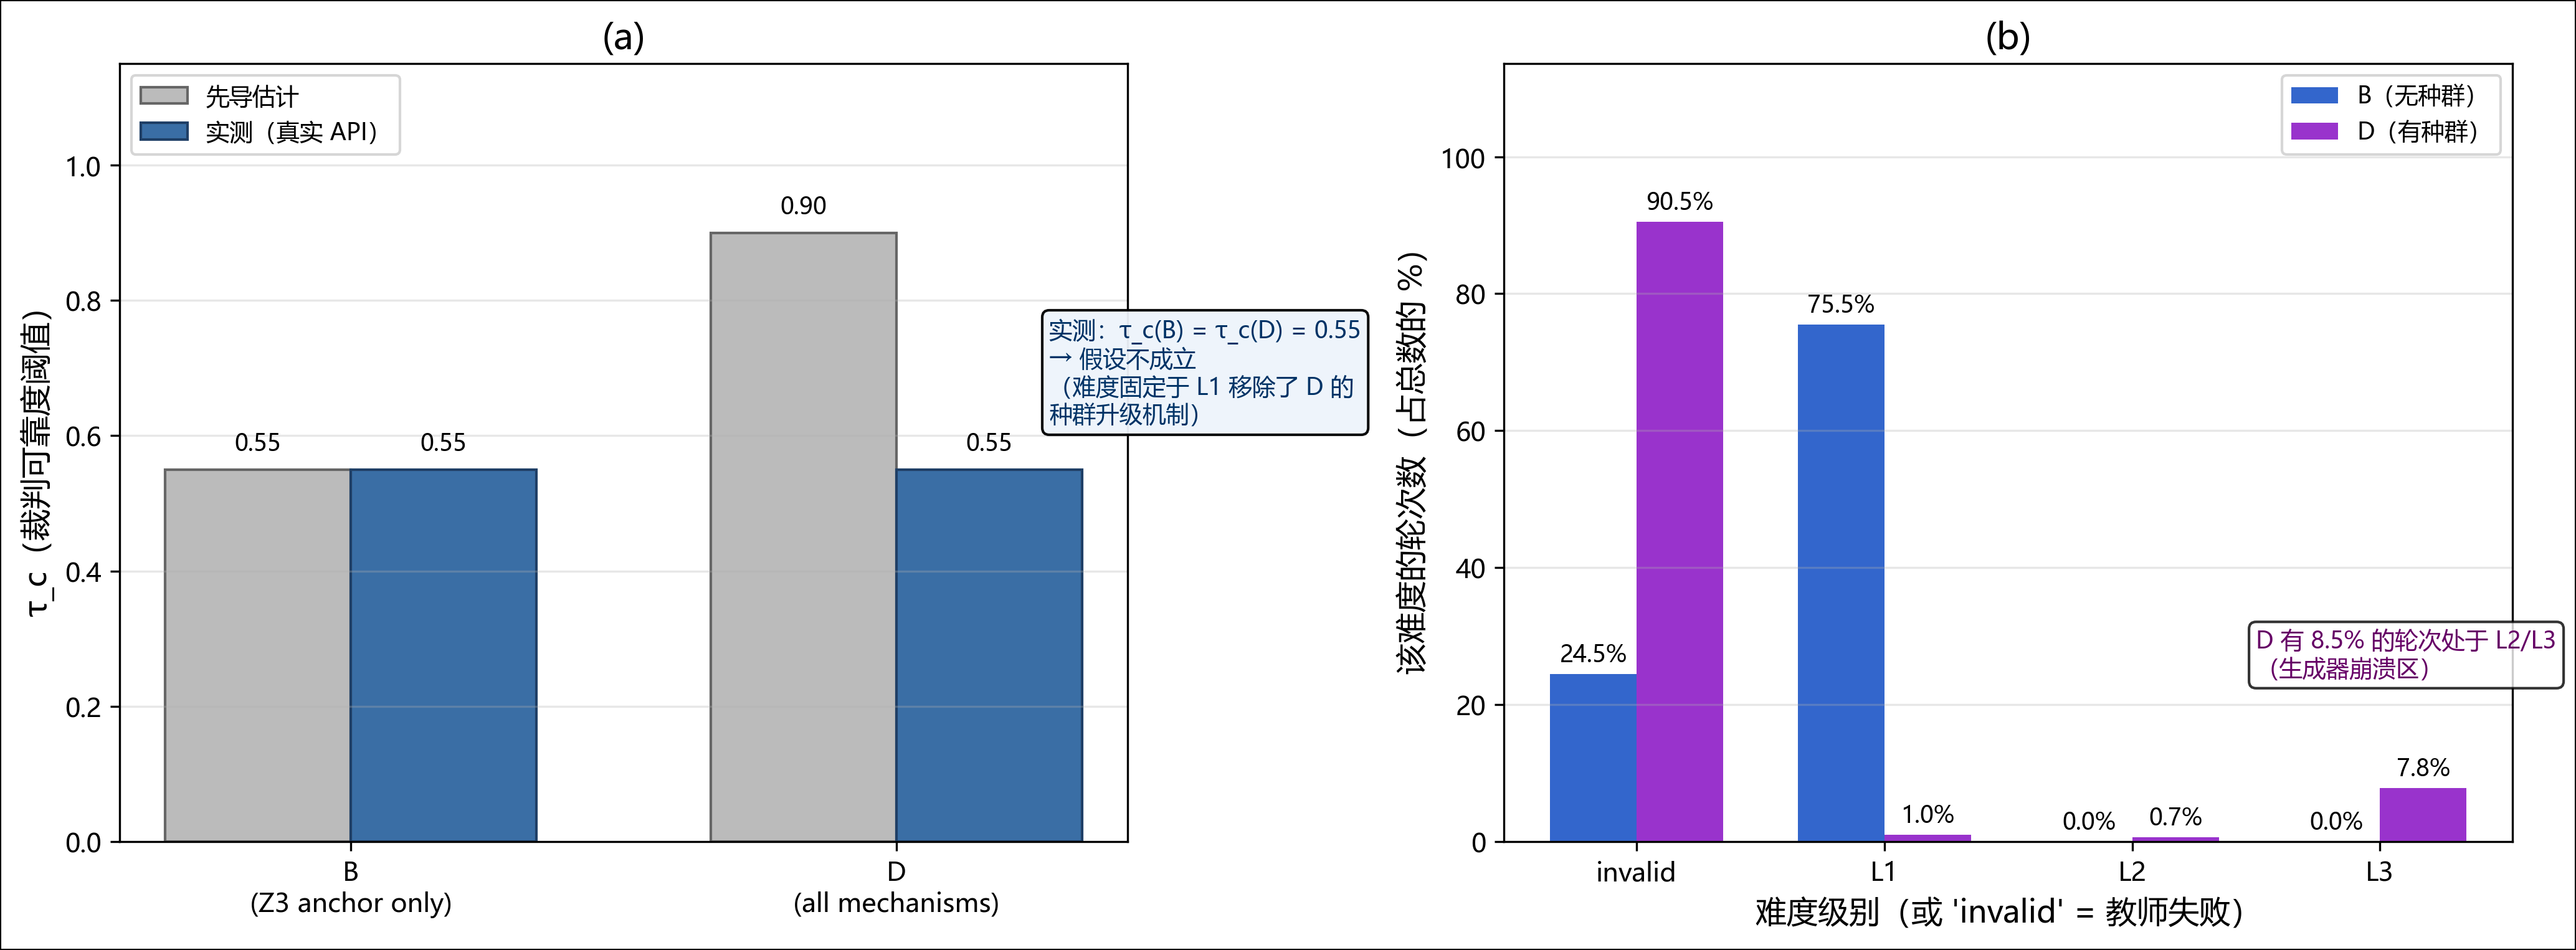
\includegraphics[width=\textwidth]{figures_zh/fig7_tau_c_gap.png}
  \caption{一次先导性估计曾给出 $\tau_c(D) = 0.90$、$\tau_c(B) = 0.55$；实测
  并未重现该差距（二者均为 0.55）。左图把先导估计与实测的 $\tau_c$ 并置
  对比，右图比较 B 与 D 的难度分布。假设
  $\tau_c(D) > \tau_c(B)$ \textit{未获支持}。}
  \label{fig:tau_c_gap}
\end{figure*}

\begin{figure*}[t]
  \centering
  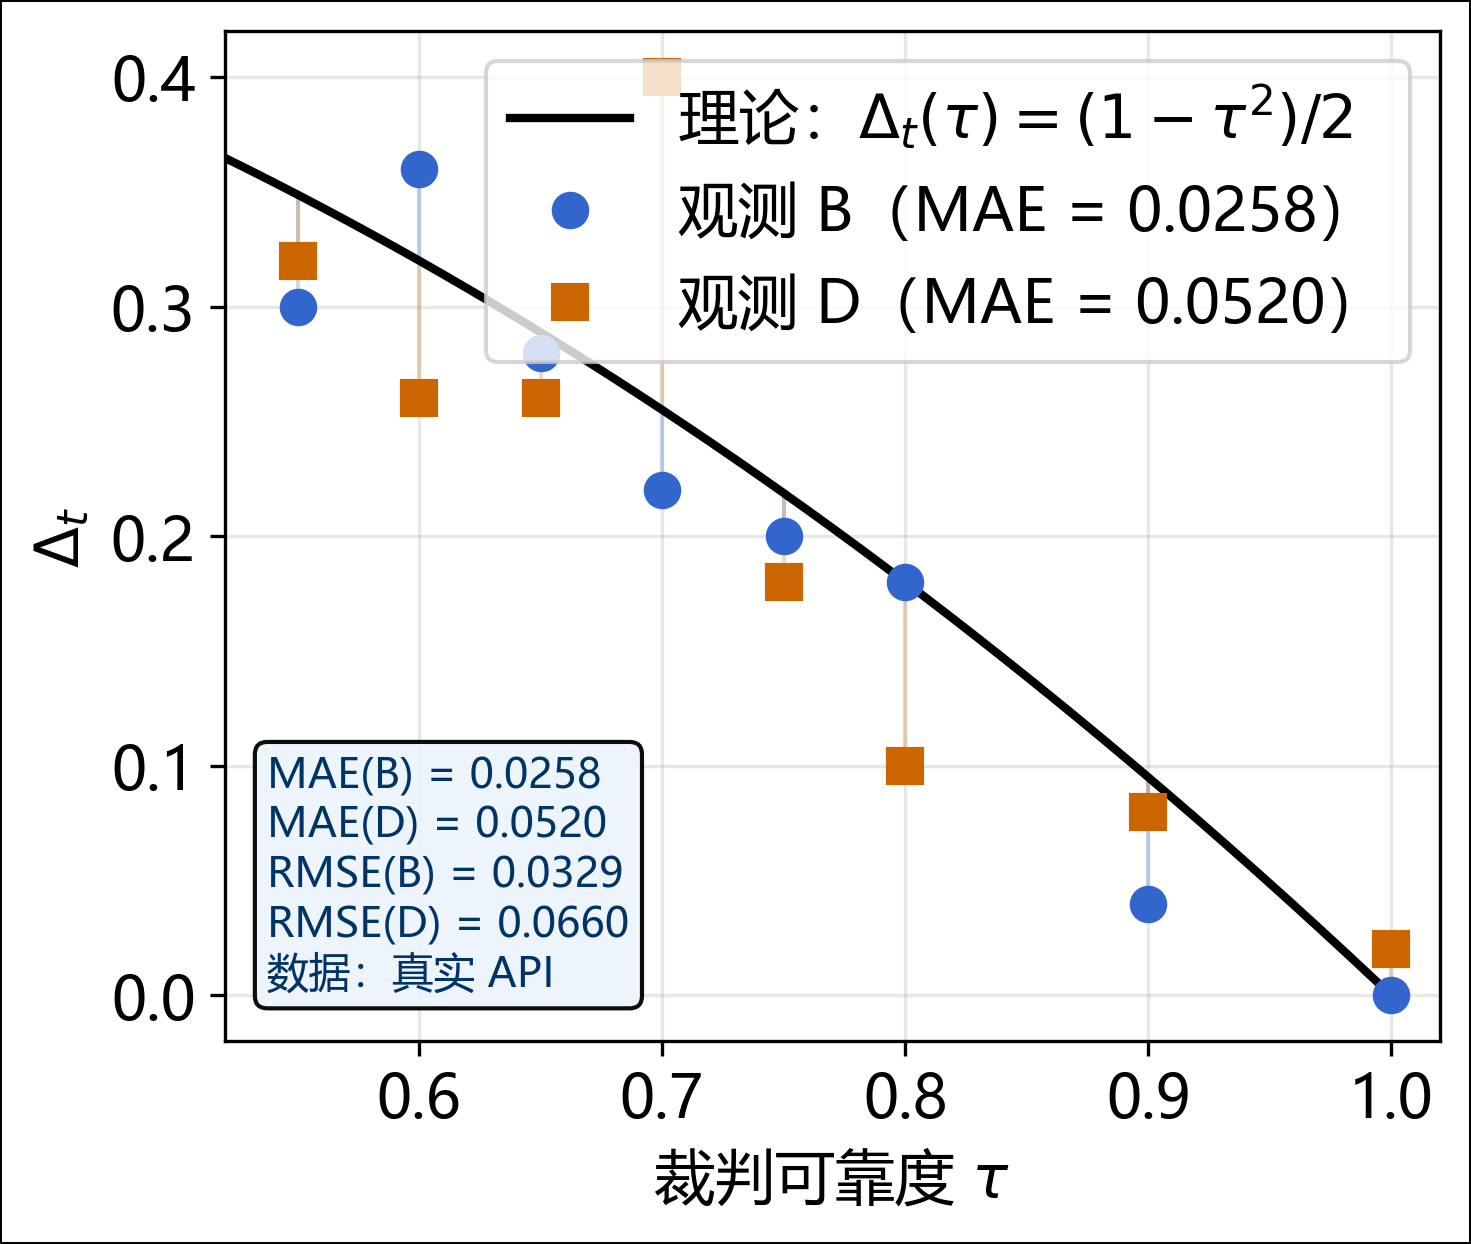
\includegraphics[width=\textwidth]{figures_zh/fig5b_tau_c_analytical.png}
  \caption{闭式解 $\Delta_t(\tau) = (1 - \tau^2)/2$ 与观测散点的对照。该
  公式不含自由参数；在每个 $\tau$ 格子上以 50 轮测得的 MAE 为 0.0258（B）
  与 0.0520（D）。当 $\tau = 0$ 时曲线锚定于 0.5 而非 1.0，这正是两次
  独立裁决所构成的二元对称性。}
  \label{fig:analytical_fit_appendix}
\end{figure*}

\begin{figure*}[t]
  \centering
  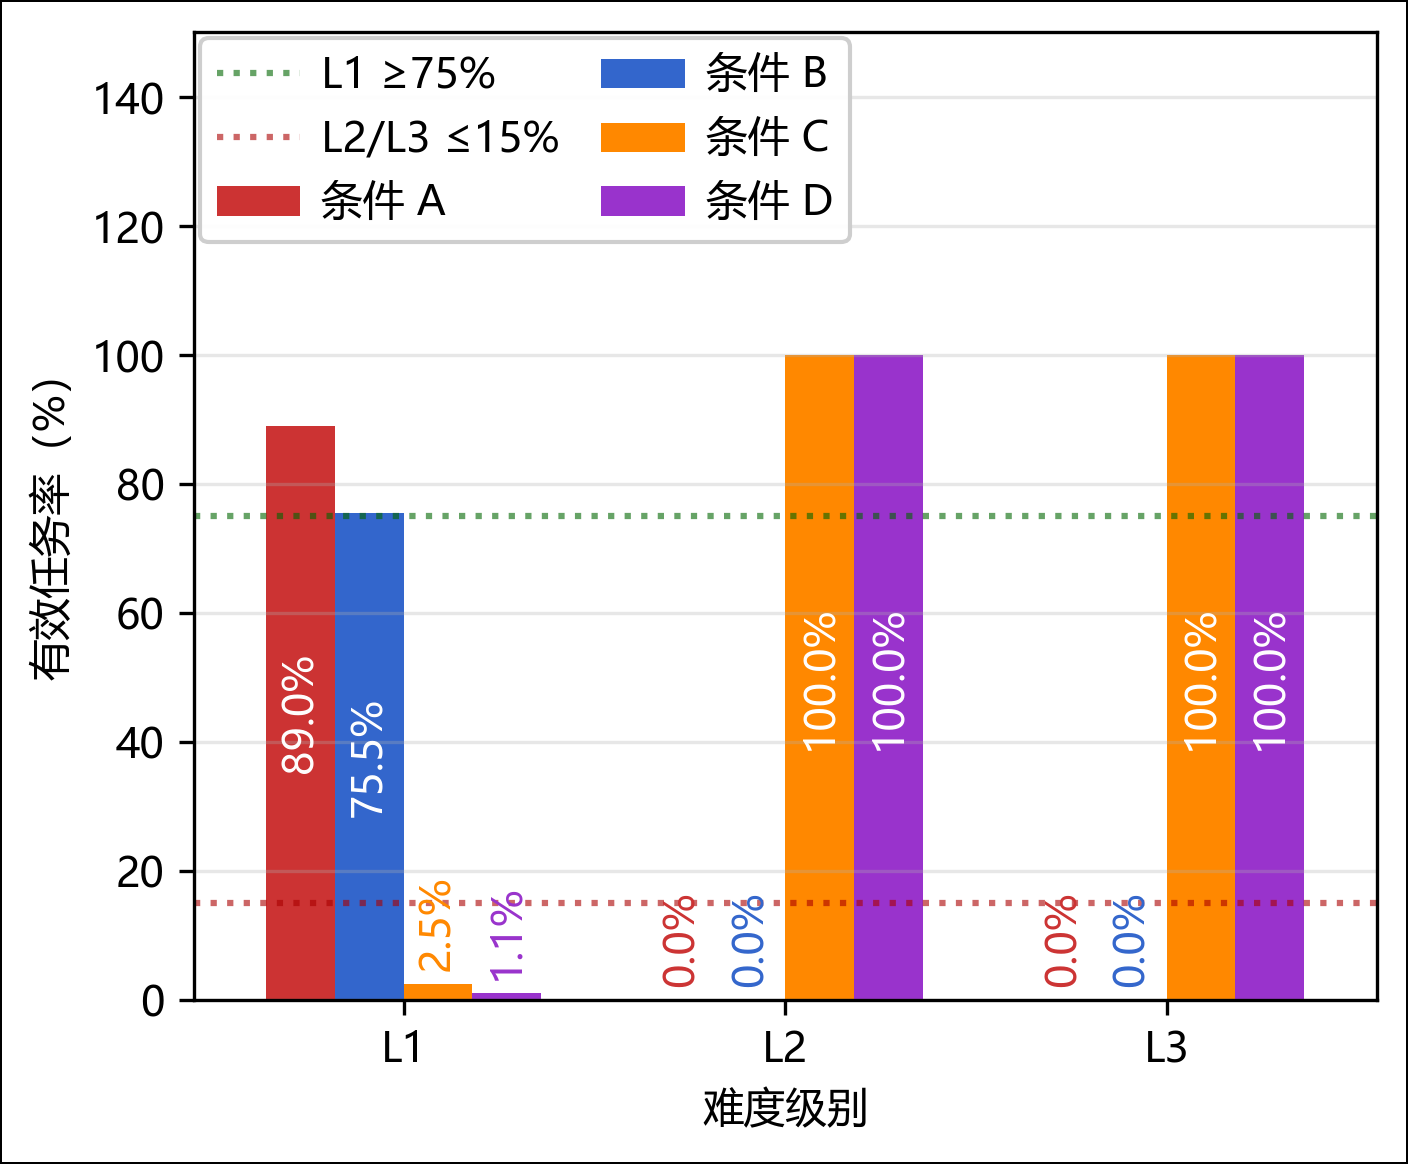
\includegraphics[width=\textwidth]{figures_zh/fig3b_validity_by_level.png}
  \caption{按难度层级划分的有效任务率。每一个抵达 L2/L3 的轮次都产出了
  有效任务：C 与 D 的 85.5\% 与 90.5\% 无效率发生在层级指派\textit{之前}，
  因为教师在 L1$\to$L2 过渡处失败，而控制器却把层级维持在高位。
  这就是伪难度陷阱。}
  \label{fig:validity_by_level_appendix}
\end{figure*}

\begin{figure*}[t]
  \centering
  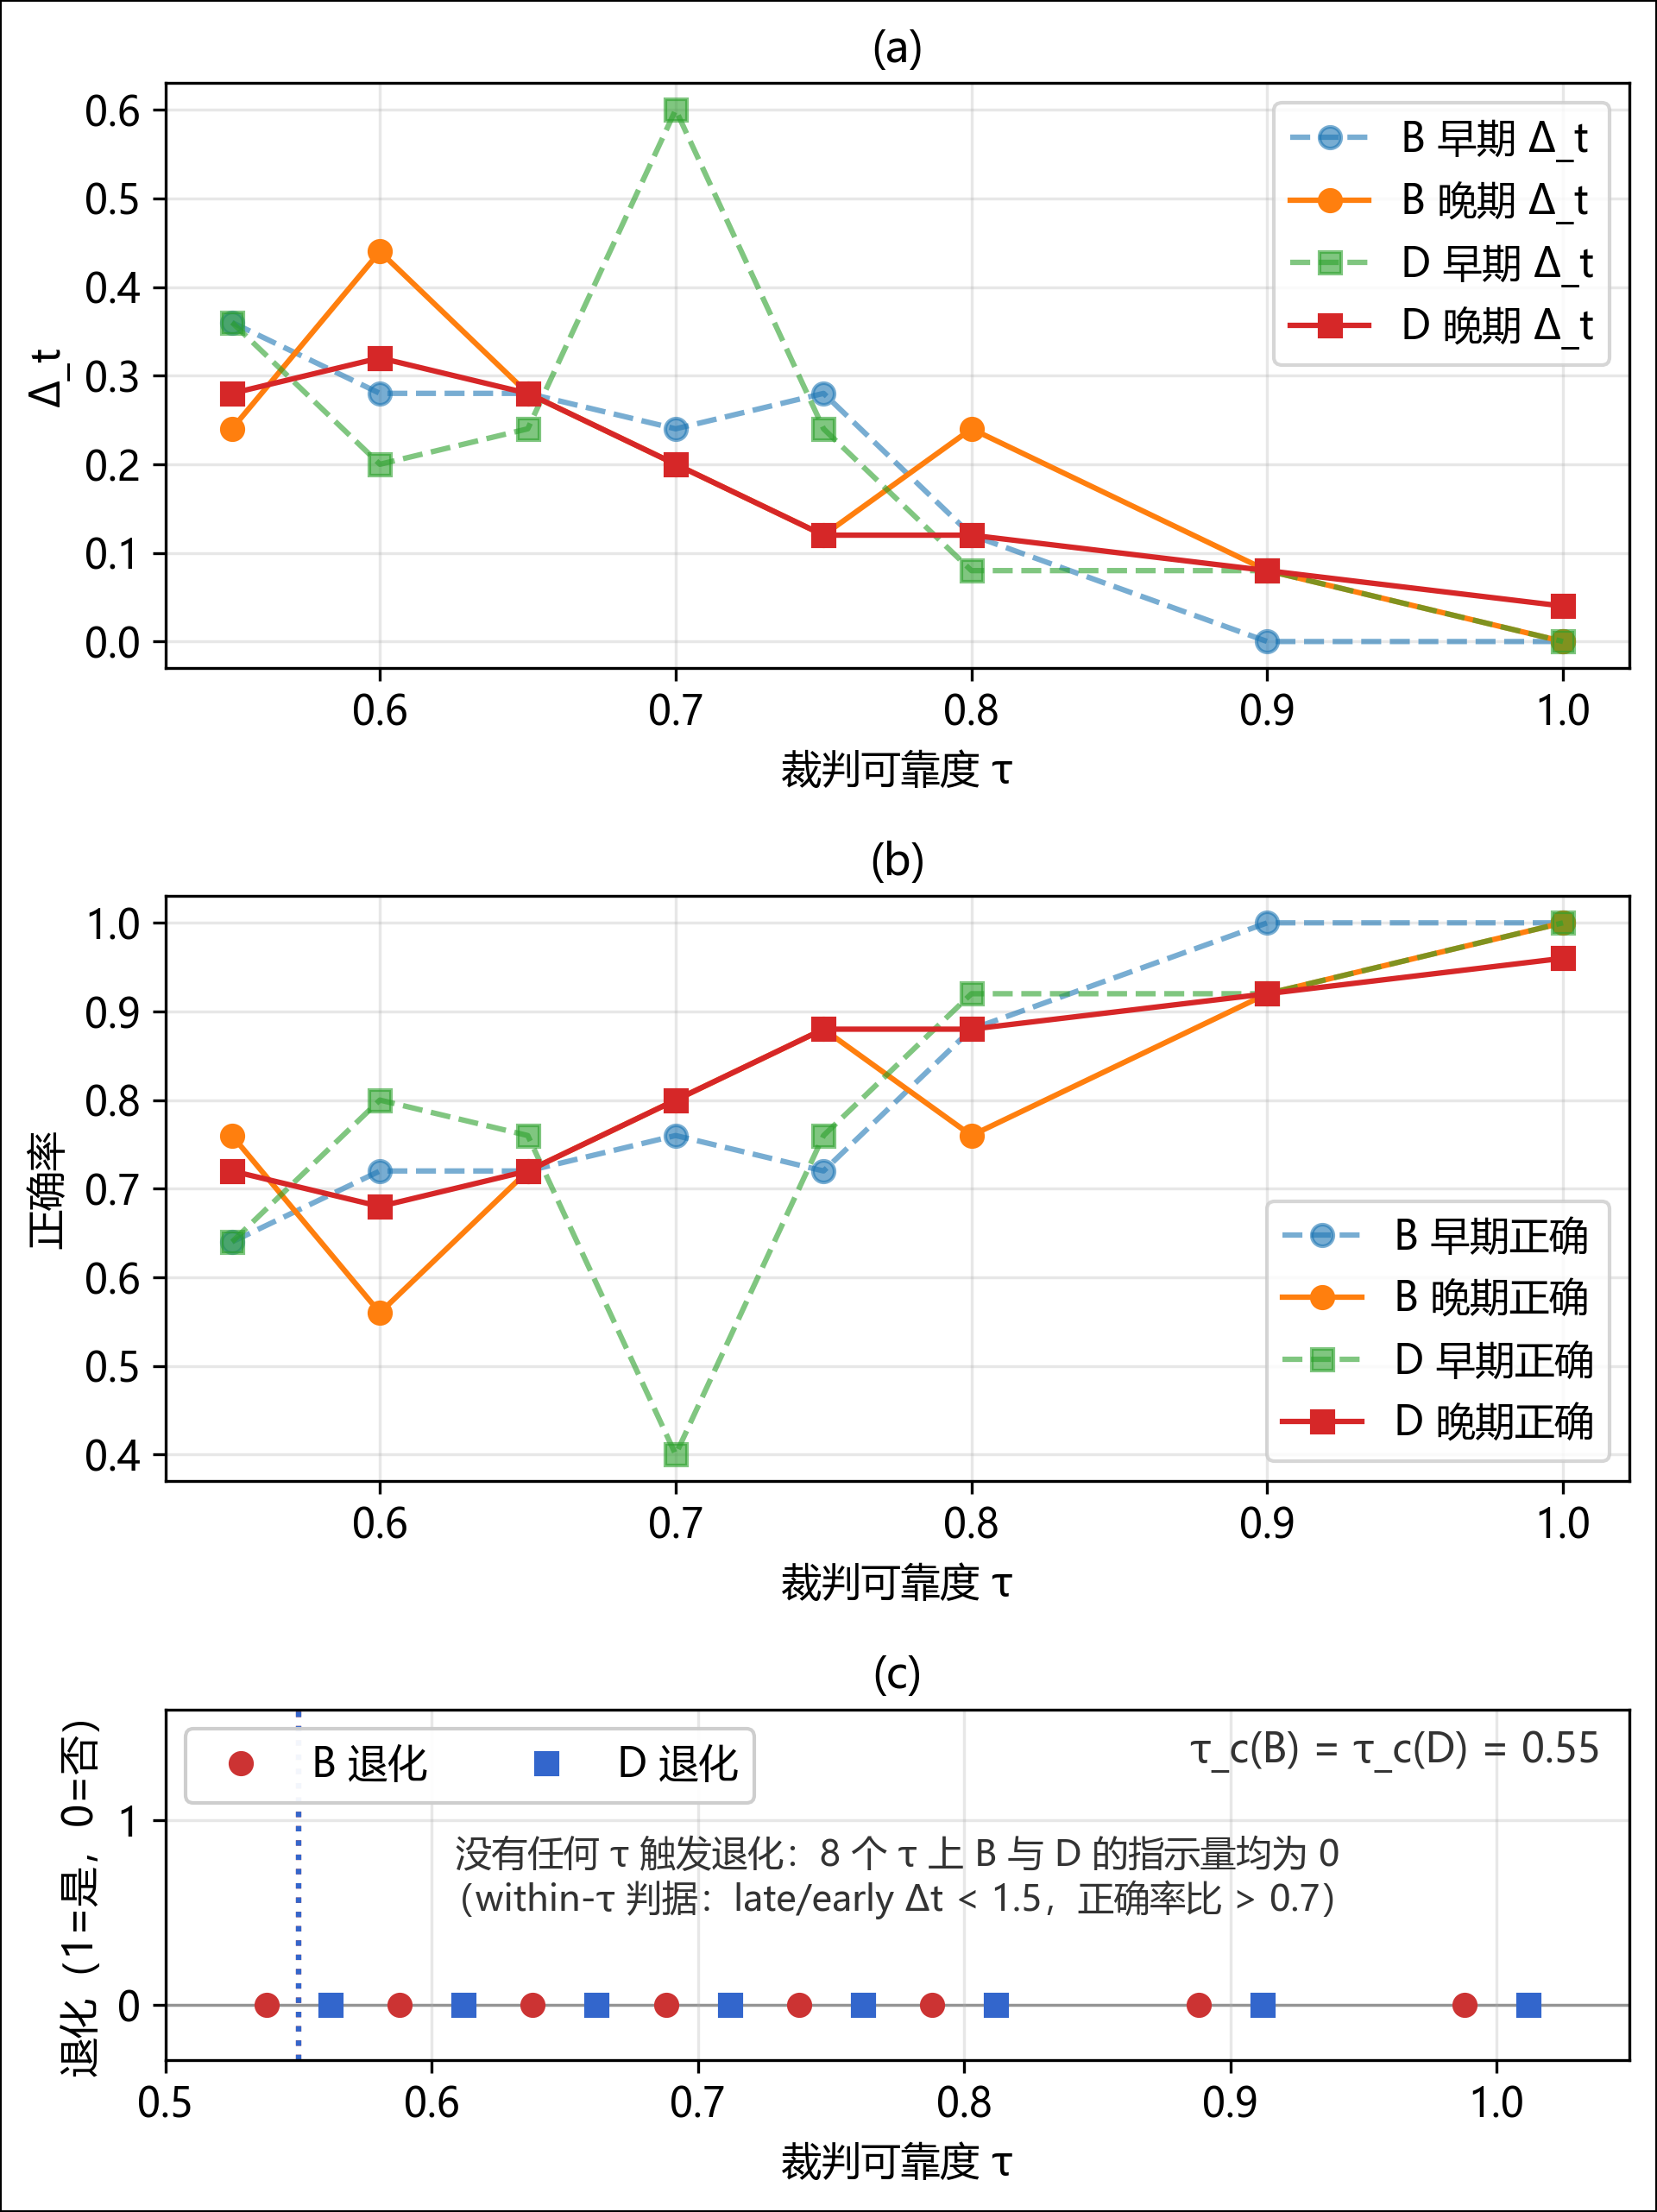
\includegraphics[width=\textwidth]{figures_zh/fig5_tau_c_curve_real.png}
  \caption{真实 API 上的 $\tau$ 梯度扫描：8 个 $\tau$ 取值 $\times$ 2 个条件（B/D）
  $\times$ 50 轮 = 800 轮。在 $\tau$ 内退化判据下没有任何 $\tau$ 取值
  发生退化，因此所报告的 $\tau_c = 0.55$ 是扫描网格的下边缘，应
  理解为上界，而非系统的容差。子图 (c) 画的是退化指示量：它在八个 $\tau$ 上
  对两个条件均为 0；两条竖线标记
  $\tau_c(B) = \tau_c(D) = 0.55$。}
  \label{fig:tau_c_curve_appendix}
\end{figure*}

\begin{figure*}[t]
  \centering
  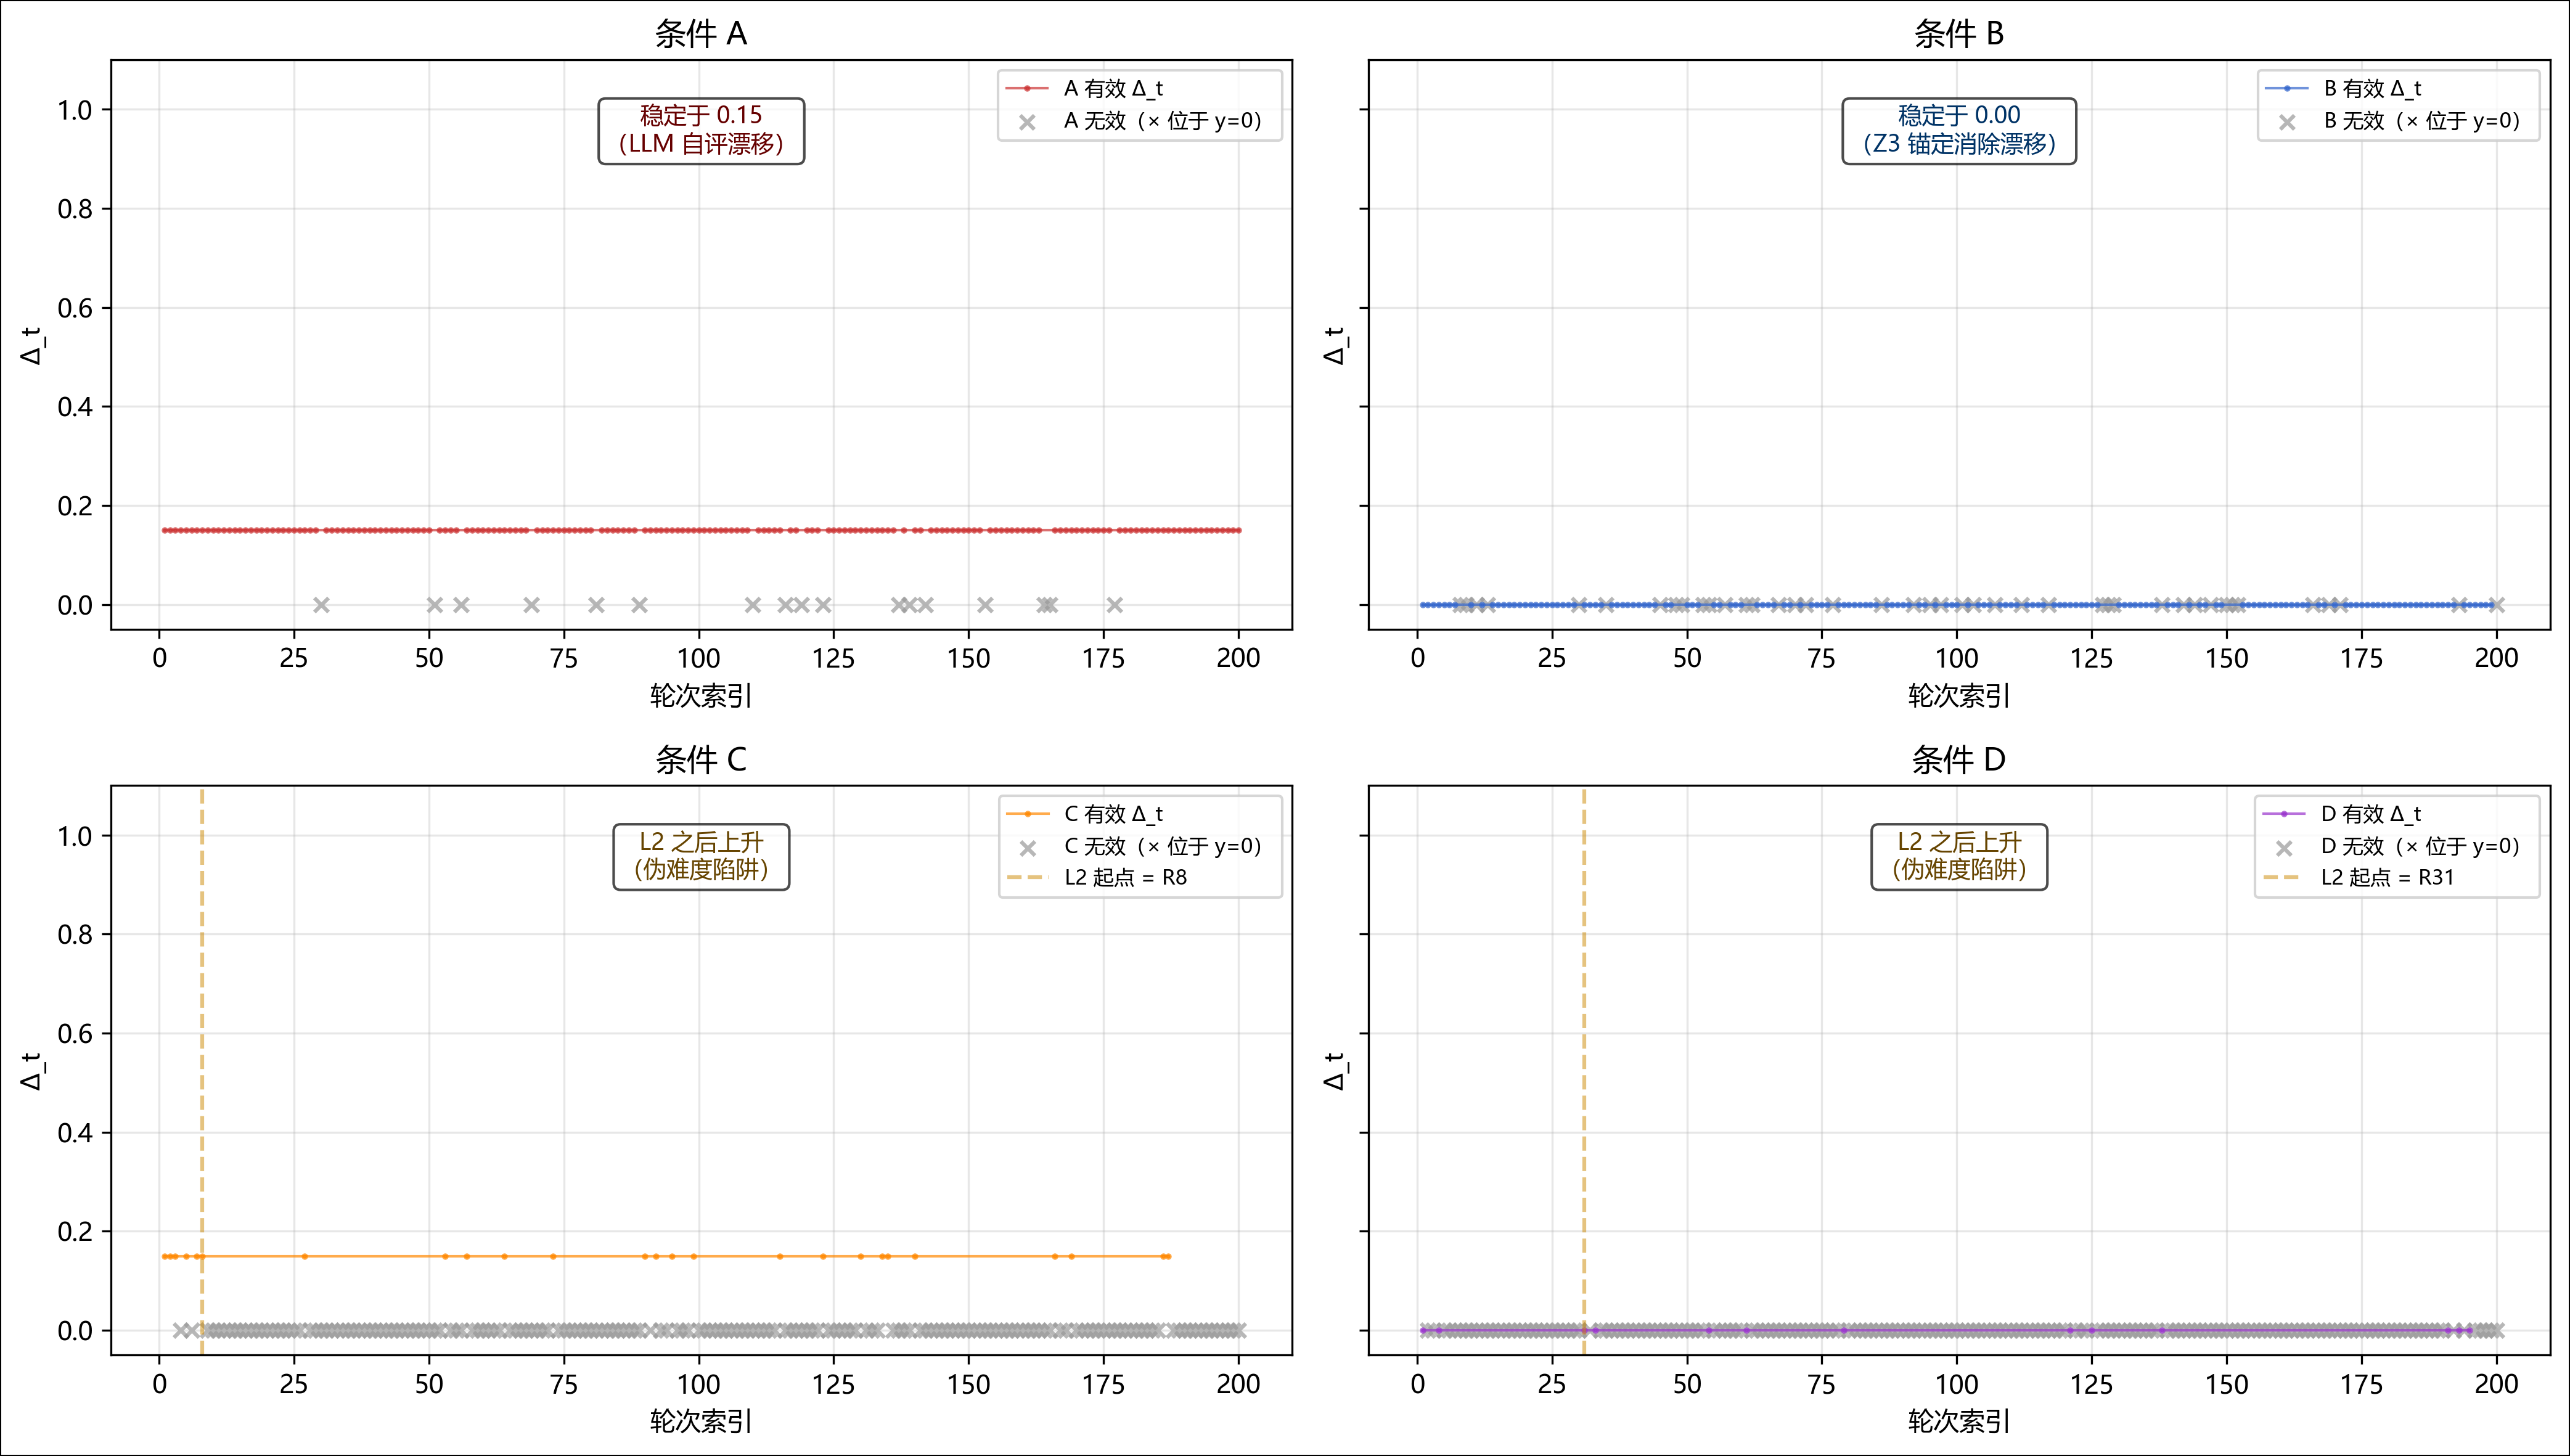
\includegraphics[width=\textwidth]{figures_zh/fig2b_delta_t_per_round.png}
  \caption{每个子图对应一个条件；无效轮次以灰色叉号标记。C/D 展示了
  L2 过渡之后的伪难度陷阱。竖线标记难度控制器首次
  提升任务层级的轮次。}
  \label{fig:delta_t_per_round_appendix}
\end{figure*}

\section{定理 1 证明梗概}

\subsection*{合成律的代数推导}

% 注：任务书要求在“附录 B”下给出本推导。在既定结构中附录 B
% 的标题是“定理 1 证明梗概”，因此这里以子节形式给出这段推导。
% 若该附录应独立成篇，可对其重命名。

令 $S = 1$ 表示该轮成功（有效任务且判定正确），否则为 $0$。令 $G = 1$
表示生成器产出有效任务，否则为 $0$；令 $J = 1$ 表示裁判正确评估
该轮次，否则为 $0$。于是 $S = G \cdot J$。由独立性（independence）：
\[
  \mathbb{E}[S] = \mathbb{E}[G] \cdot \mathbb{E}[J]
\]
\[
  1 - \Delta_t^{\mathrm{global}} = (1 - \Delta_t^{\mathrm{gen}})(1 - \Delta_t^{\mathrm{valid}})
\]
\section{被否决的备择模型}

对同一条 $\tau^{2}$ 形曲线还存在一种更简单的解释，值得明确写出，因为它最可能是读者读到这里时
会自行带入的竞争性假设。它把第二次独立判定替换为一个接受门：系统以概率 $\tau$ 接受裁判的裁断，
否则用自己的评估将其覆盖，而这一评估本身并不可靠。在该模型下，只有当\textbf{两个}事件都成功时
一轮才算正确，因此

\[
  P(\text{correct}) = \tau \cdot \tau = \tau^{2}
  \qquad\Longrightarrow\qquad
  \Delta_t = 1 - \tau^{2}
\]

该模型的三条错误路径——裁判正确但被覆盖，$\tau(1-\tau)$；裁判错误但被接受，$(1-\tau)\tau$；
以及两者皆错，$(1-\tau)^{2}$——之和为

\[
  \tau(1-\tau) + (1-\tau)\tau + (1-\tau)^{2} \;=\; (1-\tau)(1+\tau) \;=\; 1-\tau^{2}
\]

\textbf{判别性检验。}这两个模型在偏差尺度上恰好相差一个因子二，因为
$(1-\tau^{2}) \big/ \bigl((1-\tau^{2})/2\bigr) = 2$，并且它们无需任何拟合即可区分。
第~5.3 节将两者都与实测的 \texttt{correct\_rate} 作了比较：

\begin{center}
\small
\begin{tabular}{@{}llr@{}}
  \toprule
  模型 & $P(\text{correct})$ & 相对实测 \texttt{correct\_rate} 的 MAE \\
  \midrule
  两次独立判定（\textbf{本文}） & $(1 + \tau^{2})/2$ & \textbf{0.0389} \\
  裁判 $+$ 接受门（已否决） & $\tau^{2}$ & 0.2291 \\
  \bottomrule
\end{tabular}
\end{center}

在 16 个 $(\tau, \text{condition})$ 单元上，双判定模型在 13 个单元上更接近，在 2 个单元上持平，
仅在 1 个单元上落败。因此这项否决并不是在两个同样好的拟合之间做偏好选择：接受模型在 MAE 上
差了六倍。

\textbf{因子二从何而来。}接受模型没有\textit{两者皆错}的一致路径。在第~5.3 节中，只要两个裁断
\textbf{一致}，该轮即记为正确，于是概率质量分成三条穷尽的路径：两者都未被翻转、恰好一个被
翻转、两者都被翻转。第一条与第三条彼此一致，贡献的误差为零；只有中间那条概率为
$2p(1-p) = (1-\tau^{2})/2$ 的路径带有偏差。与之相对，接受模型把两者皆错的情形也计为一次错误，
正是这一点使 $\Delta_t$ 翻倍。$\tau$ 的指数由系统要求达成一致的独立判定次数决定——这是架构的
性质，而非裁判的性质。

在网格的下边缘 $\tau = 0.55$ 处，被否决的模型预测 $\Delta_t = 1 - 0.55^{2} = 0.6975$，而实测为
0.3000（B）和 0.3200（D），闭式预测为 $(1 - 0.55^{2})/2 = 0.3488$。在边界 $\tau = 0.5$ 处，
被否决的模型给出 $\Delta_t = 0.75$，而闭式给出 $0.375$——一个干净的因子二，不过扫描网格从
$\tau = 0.55$ 开始，因此在该点上并没有测量值。\textbf{本文没有任何结果使用
$\Delta_t = 1-\tau^{2}$。}

\section{数据一致性检查}
\label{app:data_consistency}

\setcounter{table}{0}
\renewcommand{\thetable}{D.\arabic{table}}

\subsection{$\Delta_t$ 的统一定义}

\[
  \Delta_t \;=\; \bigl| \text{score}(y) - \text{label}(y^{*}) \bigr|
\]

\begin{itemize}
  \item $y$：该轮提交的答案（\texttt{z3\_result.status}）；
  \item $\text{score}(y)$：系统对该答案给出的归一化评分，取值于 $[0, 1]$；
  \item $\text{label}(y^{*})$：真值标签（\texttt{sat} $= 1.0$，\texttt{unsat} $= 0.0$）。
\end{itemize}

\subsection{各条件下系统评分的来源}

表~\ref{tab:table2c_sources} 记录了在每个条件下，哪个量充当系统的评估，哪个量充当真值。

\begin{table*}[t]
  \centering
  \caption{各条件下系统评分与真值标签的来源。在 B 与 D 中，Z3 裁断与自身相比较，因此在每个有效
  轮上 $\Delta_t$ 恒为零；正是第~\ref{sec:calibers} 节的 global 口径重新引入了一个非零的平均值。}
  \label{tab:table2c_sources}
  \small
  \begin{tabularx}{\textwidth}{@{}l l l >{\raggedright\arraybackslash}X@{}}
    \toprule
    条件 & 系统评分 $\text{score}(y)$ & 真值 $\text{label}(y^{*})$ & $\Delta_t$ \\
    \midrule
    A & \texttt{llm\_self\_score}（LLM 自评分） & \texttt{expected}（Z3 真值） &
        $\bigl|\texttt{llm\_self\_score} - \text{truth}\bigr|$ \\
    B & \textbf{Z3 锚点} $=$ \texttt{z3\_result.status} & \texttt{expected} &
        \textbf{0.00} —— Z3 裁断直接采用真值，因此它是与自身相比较 \\
    C & \texttt{llm\_self\_score}，在总体上取平均 & \texttt{expected} &
        $\bigl|\texttt{llm\_self\_score} - \text{truth}\bigr|$ \\
    D & \textbf{Z3 锚点} $+$ 圆桌共识 & \texttt{expected} &
        \textbf{0.00} —— Z3 裁断是自洽的 \\
    \bottomrule
  \end{tabularx}
\end{table*}

\subsection{两种统计口径}
\label{sec:calibers}

\textbf{口径 1：valid-only $\Delta_t$（表~\ref{tab:table2b_appendix}）。}分母是
\texttt{len(records[r.valid])}。无效轮次——即教师生成失败、因而不存在真值标签的那些轮次——被
排除在外。在该口径下，A 给出 $\Delta_t \approx 0.15$，因为 LLM 自评分仅在少数轮次上偏离 Z3
真值；而 B 与 D 给出 $\Delta_t \equiv 0.00$，因为 Z3 裁断是与自身相比较的。

\textbf{口径 2：global $\Delta_t$（本附录与图~\ref{fig:delta_t_global}）。}分母是所有轮次。无效
轮次被保守地编码为 $\Delta_t = 1.0$，有效轮次保留其 valid-only 取值。在该口径下，A 升至
$\approx 0.24$，由 $11\%$ 的无效轮次推动，而 B 升至 $\approx 0.25$，由 $24\%$ 的无效轮次推动。

\subsection{表面矛盾的消解}

对照两份报告的读者会发现，一份中 A $= 0.15$、B $= 0.00$，另一份中 A $= 0.2435$、
B $= 0.2450$。二者\textbf{并不}冲突：它们是同一批轮次在上述两种口径下的读数，而
表~\ref{tab:table2c_calibers} 同时验证了两者。

\begin{table*}[t]
  \centering
  \caption{同一批轮次在两种口径下的结果。valid-only 各行即表~\ref{tab:table2b_appendix} 中的
  条目；global 各行则对每个无效轮次额外计入 $\Delta_t = 1.0$。}
  \label{tab:table2c_calibers}
  \small
  \begin{tabular}{@{}llrr@{}}
    \toprule
    口径 & 条件 & $n$ & 平均 $\Delta_t$ \\
    \midrule
    valid-only & A & 534 & 0.1500 \\
    global     & A & 600 & 0.2435 \\
    valid-only & B & 453 & 0.0000 \\
    global     & B & 600 & 0.2450 \\
    valid-only & C & 87  & 0.1500 \\
    global     & C & 600 & 0.8767 \\
    valid-only & D & 57  & 0.0000 \\
    global     & D & 600 & 0.9050 \\
    \bottomrule
  \end{tabular}
\end{table*}

本文的主表使用\textbf{口径 1（valid-only）}，而在描述伪难度陷阱时使用\textbf{口径 2（global）}，
因为在那里所关心的量恰恰是 C 与 D 使多少轮次失效。

\subsection*{从正文移出的表格}

此前位于正文中的三张表汇集于此，以便正文只保留它直接据以推理的那两张表：合成律核对
（表~\ref{tab:table4c_appendix}）、valid-only 口径（表~\ref{tab:table2b_appendix}）
与完整预算扫描（表~\ref{tab:table4cbudget_full}）。

\begin{table*}[t]
  \centering
  \caption{合成律在全部四个条件上精确到机器精度
  （2{,}400 个真实 API 轮次）。最大绝对误差 $1.11\times10^{-16}$。}
  \label{tab:table4c_appendix}
  \small
  \begin{tabularx}{\textwidth}{@{}l*{6}{>{\centering\arraybackslash}X}@{}}
    \toprule
    条件 & $n$ & $\Delta_t^{\mathrm{gen}}$ & $\Delta_t^{\mathrm{valid}}$ &
    预测 $\Delta_t^{\mathrm{global}}$ & 实测 & 绝对误差 \\
    \midrule
    A & 600 & 0.1100 & 0.1500 & 0.2435 & 0.2435 & $5.55\times10^{-17}$ \\
    B & 600 & 0.2450 & 0.0000 & 0.2450 & 0.2450 & $0$ \\
    C & 600 & 0.8550 & 0.1500 & 0.8768 & 0.8767 & $1.11\times10^{-16}$ \\
    D & 600 & 0.9050 & 0.0000 & 0.9050 & 0.9050 & $0$ \\
    \bottomrule
  \end{tabularx}
\end{table*}

\begin{table*}[t]
  \centering
  \caption{平均 $\Delta_t$（valid-only 口径）。}
  \label{tab:table2b_appendix}
  \small
  \begin{tabularx}{\textwidth}{@{}l*{5}{>{\centering\arraybackslash}X}@{}}
    \toprule
    条件 & $n$（有效） & 平均 $\Delta_t$（仅有效轮次） & 标准差 & 最小值 & 最大值 \\
    \midrule
    A & 534 & 0.1500 & 0.0000 & 0.1500 & 0.1500 \\
    B & 453 & 0.0000 & 0.0000 & 0.0000 & 0.0000 \\
    C & 87  & 0.1500 & 0.0000 & 0.1500 & 0.1500 \\
    D & 57  & 0.0000 & 0.0000 & 0.0000 & 0.0000 \\
    \bottomrule
  \end{tabularx}
\end{table*}

\begin{table*}[t]
  \centering
  \caption{对 $\Delta_t^{\max}$ 完整扫描区间的预算分解：在计入生成器瓶颈之后剩余的裁判预算，
  以及它所要求的裁判可靠性。正文以文字陈述了 $\Delta_t^{\max} = 0.60$ 的情形；此处是完整的
  扫描结果。}
  \label{tab:table4cbudget_full}
  \small
  \begin{tabularx}{\textwidth}{@{}l*{4}{>{\centering\arraybackslash}X}@{}}
    \toprule
    条件 & $\Delta_t^{\mathrm{gen}}$ & $\Delta_t^{\max}$ & 裁判预算
    & 所需 $\tau_c$ \\
    \midrule
    A & 0.1100 & 0.60 & $0.5506$ & $\ge 0$（随机即可满足） \\
    B & 0.2450 & 0.60 & $0.4702$ & 0.244 \\
    C & 0.8550 & 0.60 & $-1.7586$ & 不可达 \\
    D & 0.9050 & 0.60 & $-3.2105$ & 不可达 \\
    \midrule
    A & 0.1100 & 0.70 & $0.6629$ & $\ge 0$（随机即可满足） \\
    B & 0.2450 & 0.70 & $0.6026$ & $\ge 0$（随机即可满足） \\
    C & 0.8550 & 0.70 & $-1.0690$ & 不可达 \\
    D & 0.9050 & 0.70 & $-2.1579$ & 不可达 \\
    \midrule
    A & 0.1100 & 0.80 & $0.7753$ & $\ge 0$（随机即可满足） \\
    B & 0.2450 & 0.80 & $0.7351$ & $\ge 0$（随机即可满足） \\
    C & 0.8550 & 0.80 & $-0.3793$ & 不可达 \\
    D & 0.9050 & 0.80 & $-1.1053$ & 不可达 \\
    \bottomrule
  \end{tabularx}
\end{table*}

% ---------------------------------------------------------------------------
% 未安置的浮动体
%
% 已发布的数据包中共有 9 张表。其中七张现已各有着落（table4c
% 提供了其中两张）；剩下这两张仍需安置。请把每一张移入应当引用它的
% 那一节，并为其补上 \caption 与 \label。
%
%   table2a_delta_t_global        global 口径（在 4.2 中讨论）
%   table4b_analytical_fit        各 tau 的残差（在 5.3 中讨论）
%
% 注意：table2c_delta_t_semantics 被放置在附录 D 中，作为
% \ref{tab:table2c_sources} 与 \ref{tab:table2c_calibers}；第 4.2 节的
% 指针 \ref{app:data_consistency} 所指向的正是它。
%
% 阶段 3 把四个浮动体从正文移入附录，并删除
% 了两个正文浮动体：
%   table1（实验设置）   已删除；其内容现为第 3 节中的正文
%   table3（有效任务率） 已删除；它与
%                               \ref{fig:validity_by_condition} 重复
%   table4c（合成律）     -> 附录 D，\ref{tab:table4c_appendix}
%   table2b（valid-only dt）     -> 附录 D，\ref{tab:table2b_appendix}
%   table4cbudget               -> 正文只保留 0.60 那一段；完整
%                                  扫描结果在附录 D，
%                                  \ref{tab:table4cbudget_full}
%   table4（tau_c）              已删除；现为第 5.2 节中的一句话
%   fig5b（解析拟合）     -> 附录 A，
%                                  \ref{fig:analytical_fit_appendix}
%   fig3b（按层级的有效任务率）  -> 附录 A，
%                                  \ref{fig:validity_by_level_appendix}
% ---------------------------------------------------------------------------

\end{document}
